\chapter{Fluid flow in permeable carbonates, and X-ray imaging of fluid flow}
\section{The carbonate pore system}
Void spaces in a solid material are called pores, and such solid material with internal void spaces is called a porous medium. Carbonate rocks are the type of porous medium that studied in this thesis.

\paragraph{Porosity}
In a porous medium, the fraction of the volume of voids over the total volume is defined as the porosity ($\phi$) of the system.

Carbonate rocks are sedimentary rocks that primarily composed of carbonate minerals such as calcite and aragonite. In the context of multiphase flow in carbonate rocks, the main concern is the petrophysical properties of the pore space, such as permeability and porosity. The pore network in carbonate rocks is more complex than that found in clastic rocks, such as sandstones, which have been the focus of a greater body of research. This complexity stems from two sources, first, carbonate rocks are formed by a wide variety of biochemical processes rather than sedimentation and cementation of clastic grains. This compositional variety leads to highly heterogeneous internal structures and therefore complex distribution of permeability and porosity. Second, the mineralogy of carbonate rocks, mostly calcium magnesium carbonates, is more prone to diagenetic alteration and modification than sandstones. Diagenesis can drastically alter the internal structure of the carbonate rock and lead to even higher heterogeneity. Oppositely, diagenesis process of dolomitisation might overprint a carbonate rock, either locally or on a large scale, with a much simpler pore structure and distribution. Therefore, unlike clastic rocks that barely undergo any alteration in comparison to that seen by carbonates, the shape, size and spatial distribution of porosity in carbonate rocks span across a much wider range. A good example of this key difference with sandstone is well illustrated by \citet{van2013modelling} who modelled the permeability evolution of carbonate rocks. The research used a pore-scale modelling approach to investigate the impact of different diagenetic events on porosity and permeability evolution of carbonate rocks. The results display several ‘diagenetic tipping points’ where the permeability decrease is drastically larger than expected associated with porosity decrease. Pore networks in carbonate rocks are complex and have received less attention experimentally than sandstones. However, this has begun to change in the last few years as the importance of carbonates has become increasingly recognised. The experimental, analytical and modelling tools also have been refined and improved, in part through studies on sandstones, so that they are readily to be applied to carbonates.

\subsection{The origin and classification of porosity in carbonate rocks}
Carbonate sediments are mainly derived from four sources \citep{stehli1961mineralogy}: 1) skeletal remnants of marine organisms, 2) physiochemical precipitation from sea water, 3) bacterial precipitation and 4) detritus of pre-existing carbonate rocks. Mineralogy composition of carbonates are characteristically composed of calcite, aragonite or dolomite, or a mixture of phases. 

The porosity in carbonate rocks is created by depositional and post-depositional processes. \citet{murray1960origin} categorised the carbonate porosity into three types. 

\paragraph{Primary porosity} 
The first type is called primary porosity, which refers to the pores created by depositional process. The primary porosity might have been slightly altered by post-depositional processes such as compaction, pressure solution, sementation and dissolution, but the original pore fabric is intact and recognisable. Accroding to \citet{murray1960origin} the depositional processes mainly include three type of carbonate sediments: framework, muds and sands. 

\paragraph{Framework} are carbonate sediments that were originally rigidly bound. The framework can be either organic or inorganic, such as interlocking carbonate crystals and skeletal debris of organisms. 

\paragraph{Muds} are fine carbonate particles known as lime muds. The particles can be either (bio)chemically precipitated fine carbonate crystals, or fine grains that originated from larger carbonate rock debris. The size of mud particle is commonly less than 10 \textmu m.

\paragraph{Sands} are carbonate sediments deposited as sorted sands or gravels. Such carbonate particles are largely produced locally and physio-chemically, for example oolites and pellets. The lack of transport distance leads to often poorly sorted carbonate sands, therefore the pore size distribution of carbonate sands can be much heterogeneous than its terrigeneous counterpart sandstone.

The primary porosity is likely to be altered by post-depositional process. The pore space can be reduced by compaction, sementation and crystal overgrowth, they also can be enlarged by pressure solution and dissolution.

\paragraph{Sucrose dolomite} 
The second porosity type in carbonate rocks is sucrose dolomite. This type of porosity is created by post-depositional dolomitisation on the pore surface. The euhedral and subhedral dolomite crystals tend to interfere with each other and only slightly welded at points of contact, forming inter-crystalline pore space that resembles to the surface of lump sugar.

\citet{murray1960origin} stated that sucrose dolomite pores are quantitatively the most important for the oil and gas production in North American reservoirs. The dolomite crystal size ranges from less than 5 \textmu m to over 100 \textmu m, most commonly 25-50 \textmu m. The carbonate solution needed for crystallising new dolomite rhombs can be either derived from outside of the system, or from locally dissolved pre-existing carbonates. If the source is newly introduced into the system, the bulk porosity should decrease. If the carbonate source is locally provided, it means new dolomite crystals are compensating the voids created by dissolution, in this case porosity should increase by a little due to replacing calcite with denser dolomite. 

\paragraph{Secondary vugs} 
The third porosity type is secondary vugs. They are void space formed by post-depositional dissolution process. Vugs can be formed by dissolution of replacement minerals, often anhydrite \citep{murray1960origin}. Vugs can be formed by selective dissolution of carbonate minerals, such as aragonite, dolomite or chert. Selective dissolution can produce an interconnected vug network that resembling to inter-particle porosity. Vugs can be also formed by fracture. Although the contribution to porosity from fracture is usually less than 1\%, but the contribution of interconnected fractures to multiphase fluid flow should be recognised \citep{murray1960origin}.

\subsubsection{Carbonate pore system classification}
Two of the mostly used classification schemes for carbonate rocks are \citet{folk1959practical}'s and \citet{dunham1962classification}'s classification. Both Dunham and Folk's classification are based on the lithological texture of carbonate rocks, however the main concern of this study area is mainly the geometry and volume of the void spaces (e.g. porosity, tortuousity and aspect ratio etc.) and the physical properties of the surface of the void spaces (e.g. wettability and roughness) in the carbonate rocks, regardless of the composition and texture of the solid parts. Therefore, a more suitable type of classification schemes is the pore-type based classification.

\paragraph{Matrix and visible pores}
\citep{archie1952classification} first introduced a classification scheme concerning the petrophysical attributes of carbonates. Archie's classification consists of two parts: the texture of the matrix and the character of the visible pore structure. He categorised a carbonate matrix into three types based on the texture: crystalline, chalky and granular, and described the appearance of the three matrix types of hand sample and under microscope. The visible pore size are classified into four groups A to D based on their size. Archie's classification is the first of its kind, and the only method at that time to estimate the porosity of an uncored well.

\paragraph{Fabric selectivity}
\citet{choquette1970geologic} introduced the important concept of fabric selectivity for pore system classification. Solid constituents of carbonate rocks can be primarily formed during sedimentation processes, or secondarily formed during diagenetic events. These primary and secondary solid constituents are collectively defined as 'fabric elements'. The degree of dependence of the pore space with the fabric elements is defined as fabric selectivity. If the pore space has a dependent relation with the fabric elements, the pore space is referred to as fabric-selective, if such a relation can not be established, the pore space is not fabric-selective. Fabric-selective pores are for example interparticle pores, intraparticle pores, intercrystal pores, moldic pores etc. Non-fabric-selective pores are for example fractures, channels and vugs. Some pores can be either fabric-selective or non-fabric-selective, for example breccia, boring, burrow and shrinkage (Fig.\ref{fabricselectivity}). 

\begin{figure}[htbp]
  \centering
  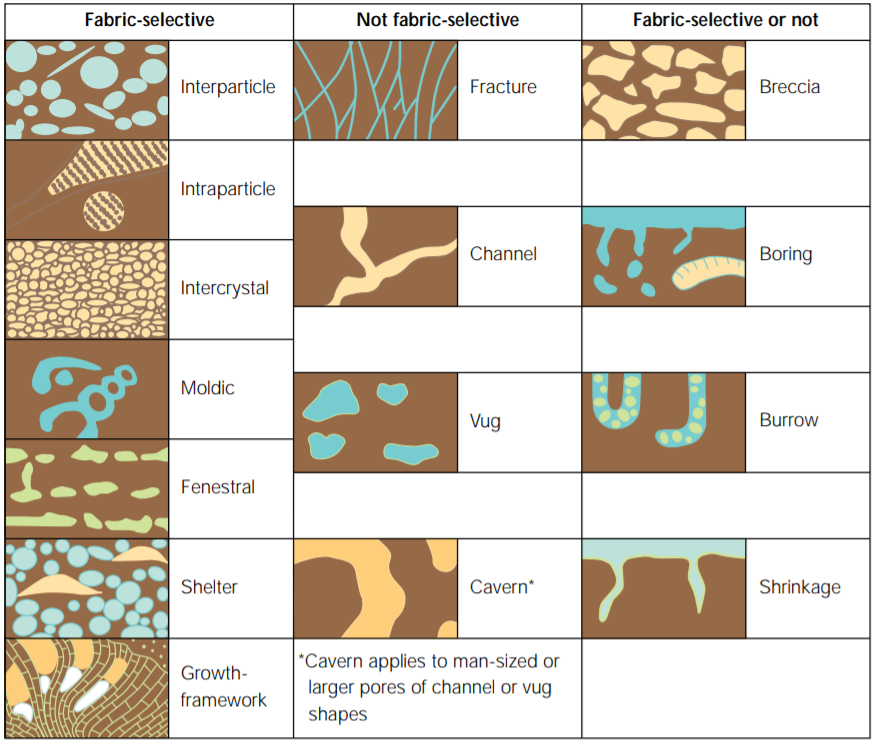
\includegraphics[width=1\textwidth]{\dir/figs/fabricselectivity}
  \caption{Carbonate rock pore classification by fabric selectivity. Left column: Fabric-selective pores. Middle column: Non-fabric-selective pores. Right column: possibly frabric-selective pores. Adapt from \citep{akbar1995classic}.}
  \label{fabricselectivity}
\end{figure}

\paragraph{Interparticle and vuggy pores}
\citet{lucia1995rock} developed a carbonate classification , built on his own work in 1983 \citep{lucia1983petrophysical} that taken both fabric selectivity and petrophysical properties into consideration. This classification serves better for reservoir classification because it focuses more on the goal of describing the spatial distribution of petrophysical parameters such as porosity, permeability and fluid saturation. This classification scheme is summarised in Fig.\ref{interparticle} and Fig.\ref{vuggy}. Pores in carbonate rocks are categorised into two main groups, interparticle pore space and the vuggy pore space. The interparticle pore space is divided further into three sub-categories based on size and sorting of grains and crystals, termed rock-fabric/petrophysical classes (Fig.\ref{interparticle} lower). These three classes define permeability and saturation fields and therefore can be used together with other data to relate petrophysical properties with geological observations \citep{lucia1995rock}.The fabrics are divided into grain-dominated fabric and mud-dominated fabric. For the vuggy pore space, two sub-categories are divided based on vug interconnection, namely separate-vug pores and touching-vug pores. The fabrics are divided into grain-dominated, mud-dominated and grain-mud-dominated fabrics (Fig.\ref{vuggy}). \citet{lucia1995rock}'s classification improved Archie's \citep{archie1952classification} by incorporating \citep{choquette1970geologic}'s fabric-selectivity concept.

\begin{figure}[htbp]
  \centering
  \includegraphics[width=.9\textwidth]{\dir/figs/lucia}
  \includegraphics[width=.9\textwidth]{\dir/figs/lucia3}
  \caption{Interparticle pore space from the classification scheme of \citet{lucia1995rock}. Upper figure: Carbonate interparcitle pores categorised into two main groups: 1) grain-dominated fabric and 2) mud-dominated fabric. Further categorised into sub-groups by percentage of interparticle porosity. Lower figure: Petrophysical classes of the upper figure. The upper figure is re-divided into three classes: class 1) grain-dominated grainstone. Class 2) grain-dominated packstone. Class 3) mud dominated packstone/wackestone/mudstone. Adapt from \citep{lucia1995rock}.}
  \label{interparticle}
\end{figure}

\begin{figure}[htbp]
  \centering
  \includegraphics[width=.9\textwidth]{\dir/figs/lucia2}
  \caption{Vuggy pore space from the classification scheme of \citet{lucia1995rock}. Vuggy pore space of carbonate rocks are divided into separate-vug pores and touching-vug pores. Two sub-divisions of separate-vug pores are grain-dominated fabric pores and mud-dominated fabric pores. Image adapted from \citep{lucia1995rock}.}
  \label{vuggy}
\end{figure}

\paragraph{Porosity Distribution Classification}
\citet{lonoy2006making} improved Lucia's classification by introducing the consideration of porosity distribution. L{\o}n{\o}y's classification of carbonate pores is based on three criteria, namely pore type, pore size and pore distribution. Six pore types are defined: Interparticle, intercrystalline, intraparticle, moldic, vuggy and mudstone microporosity. Pore sizes are divided into three categories: micropores, mesopores and macropores. The defined range of the pore size types are dependent on pore types. Pore distribution has two classes, uniform and patchy. Combining these three criteria L{\o}n{\o}y had summarised 20 types of pore fabrics (Fig.\ref{lonoy}).

\begin{figure}[htbp]
  \centering
  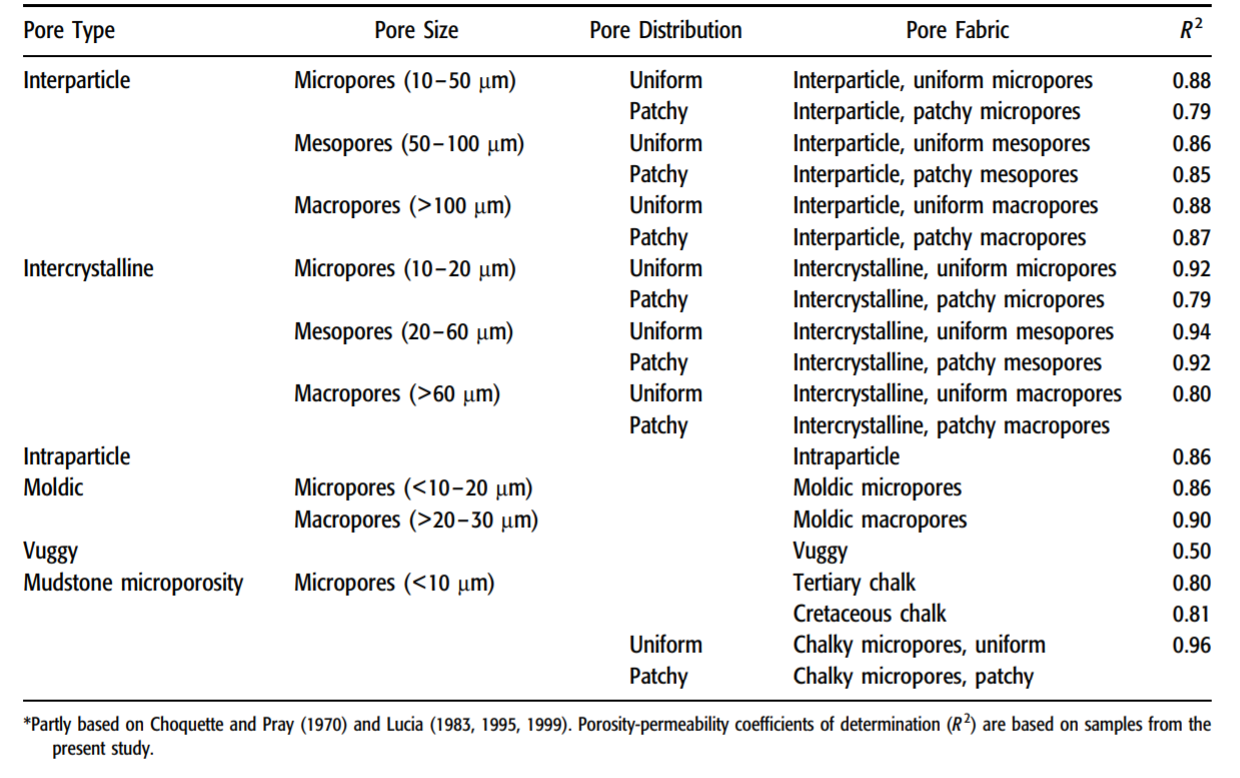
\includegraphics[width=.9\textwidth]{\dir/figs/lonoy2006}
  \caption{L{\o}n{\o}y's classification. Carbonate pores are classified based on pore type, pore size and pore distribution. 20 types of carbonate pore structures are classified. The trend line coefficients of determination $R^2$ of each pore class were significantly improved compared to other classifications, indicating good separability of the classification scheme. Adapted from \citet {lonoy2006making}.}
  \label{lonoy}
\end{figure}

\section{Multiphase flow in porous media}
In this section, basic concepts of multiphase flow in porous media, in a general context, will be introduced. Before discussing multiphase fluid flow, we first consider a porous medium with only one fluid that flows in.

\subsection{Permeability}
The porous medium has an intrinsic property called permeability, it measures the capacity of porous medium to transmit a particular fluid \citep{peters2012overview}. According to the review by \citet{honarpour2018relative}, permeability of a porous medium is defined as following: 

\textit{``A porous material has a permeability of 1 D when a single-phase fluid with a viscosity of 1 cP (10$^-3$ Pa·s) completely saturates the pore space of the medium and will flow through it under viscous flow at the rate of 1 $cm^3/sec/cm^2$ cross-sectional area under a pressure
gradient of 1 atm/cm''} 

Permeability has the units of length squared, which is $m^2$ in SI unit. However conventionally the Darcy (D) is used as the unit for permeability. The Darcy by definition is not based on a conversion to SI units, it is converted to SI unit that $1D \approx 10^{-12} m^2$ with sufficient accuracy for engineering purposes. The Darcy is a very large unit, the more common unit for permeability in rocks is milliDarcy (mD). One reservoir rock with the permeability of below 1 mD is conventionally classified as 'low permeability', 1-10 mD is 'fair permeability' and 10-100 mD will be 'high permeability'.

\subsection{Darcy's law}
When a single phase fluid flows in a porous medium, its flow rate can be described by Darcy's law. French engineer Henry Darcy \citeyear{darcy1856public} first introduced this empirical relationship to describe flow in sand filters for fountains. The flow rate is linked to the viscosity and density of the fluid itself, as well as the permeability of the pore system. The general form of Darcy's law was first proposed by \citet{nutting1930physical} and \citet{wyckoff1933measurement} as:

\begin{equation}
    \mathbf{q}=-\frac{K}{\mu }(\nabla P-\rho \textbf{g})
\end{equation}

\mathbf{q} denotes the Darcy velocity, i.e. the volume of fluid flowing per unit area (both solid and void). K is the permeability of the porous medium.$\nabla$ P is the pressure gradient and \textrho \textbf{g} is the unit weight of the fluid. Darcy's law is essentially the empirical expression of a simplified Navier-Stokes equation that governs fluid flow. The mathematical expression will not be presented here for simplicity but will be introduced later.

\subsection{Interfacial tension, contact angle and wettability}
\subsubsection{Interfacial tension}
We now consider a system of two immiscible fluids contacting with each other, without a porous medium. When two fluid phases stabilised, the fluids adjust their shape to achieve minimum contacting surface area because of interfacial tension. Interfacial tension, \textsigma, is defined as the energy per unit area of the surface between the phases \citep{blunt2017multiphase}. The energy is sourced from penalty of breaking the inter-molecular interactions within each phase and creating a surface instead. The energy is low between two immiscible fluids with similar inter-molecular bonding (e.g. oil and a high-pressure hydrocarbon gas). The energy is high between two immiscible fluids with different inter-molecular bonding (e.g. air and mercury). The physical explanation of interfacial tension is the competing van der Waals inter-molecular forces inside each phase and between the phases \citep{blunt2017multiphase}. The effect of interfacial tension can be observed in nature. For example, ignoring gravity and buoyancy, an air bubble in water is a round sphere when it is stabilised. This is because sphere has the minimum surface area for a fixed volume. 

\subsubsection{Contact angle}
We now consider two contacting immiscible fluid phases on a solid surface. When two fluid phases stabilised, the interface between the two fluids is usually a smooth surface. Fig.\ref{contactangle} shows a conceptual illustration of how a water droplet resides on a solid surface, surrounded by the second fluid phase-air. The interface between water and air forms a surface. The surface has a curvature $\kappa$, and the radius of the curvature $r=\frac{1}{\kappa}$. For less ideal case, the interface can be irregular and consisted of several curvatures.

\begin{figure}[htbp]
  \centering
  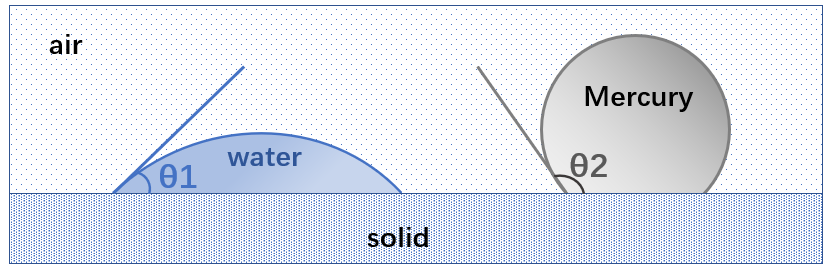
\includegraphics[width=1\textwidth]{\dir/figs/contactangle}
  \caption{Schematic illustration of contact angles measured for a water droplet $\theta 1$ and a mercury droplet $\theta 2$ on a water-wet solid surface (surrounded by air).}
  \label{contactangle}
\end{figure}

At the point where the two fluids are in contact with the solid, an contact angle $\theta$ is formed \ref{contactangle}. The contact angle is dependent on the interfacial tension between the two fluids, and between each fluid and the solid. The contact angle is conventionally measured for the denser fluid phase \citep{blunt2017multiphase}, in this case water, for a valid range from $0^{\circ}$ to $180^{\circ}$. Besides direct measurement, the value of contact angle can be also derived from the Young equation, which will be introduced later.

\subsubsection{Wettability}
From the value of the contact angle, the wettability of the solid can be determined. Wettability indicates the tendency of one fluid phase to spread over the solid surface in presence of another fluid \citep{craig1971reservoir}. In the context of this study, the two fluids are oil and brine, if more generically organic phase, aqueous phase or gaseous phases are concerned for wettability. The contact angle is measured through the water phase because of higher density. If the contact angle $0^{\circ}<\theta<90^{\circ}$, the solid material is water-wet. If the contact angle $\theta=90^{\circ}$, the solid material is neutrally/intermediately-wet. If the contact angle $90^{\circ}<\theta<180^{\circ}$, the solid material is oil-wet. For extreme cases, if the contact angle $\theta=0^{\circ}$, the solid is completely water-wet and for $\theta=180^{\circ}$ the solid is completely oil-wet \citep{blunt2017multiphase}. When referring to the wettability of a porous medium, it refers to the contact angle distribution throughout the pore space . 

In practice, in a real porous rock, the wettability is more complex than in theory. The solid surface can not be absolutely flat and smooth but has some degree of irregularity and roughness, and the mineral composition can be different from place to place. There may be presence of a surfactant in the fluid or deposited on the surface of the solid. The composition of fluids are also complex. In deep aquifers and oilfields, the aqueous phase is a highly saline solution called brine. The composition of a crude oil is even more complex, involving a mixture of hydrocarbon compounds like alkanes, naphthenes and other aromatics and heavy asphaltenes \citep{westlake1974biodegradability}. The fluid wettability might also be altered by soluble gas \citep{lee1974water}. For the above reasons, the wettability in real reservoir/aquifer rock is often non-uniform, wettability can change from pore to pore or even within one single pore.

\citet{mcdougall1995impact} classified the non-uniform wetting systems into two categories. The fractionally-wet system and a mixed-wet system (Fig.\ref{wetsystem}). A fractionally-wet system (Fig.\ref{wetsystem}A) has the wettability distribution of both fluids for all range of pore radius. That is to say, oil-wet pores can be found in all size of pores. A mixed-wet system (Fig.\ref{wetsystem}B) has the wettability distribution that is separated by a specific threshold of pore radius. Pores that are smaller than the threshold radius are water-wet and pores sized above the threshold radius are oil-wet. Such wettability distribution could be a result of wettability alteration which will be discussed later.

\begin{figure}[htbp]
  \centering
  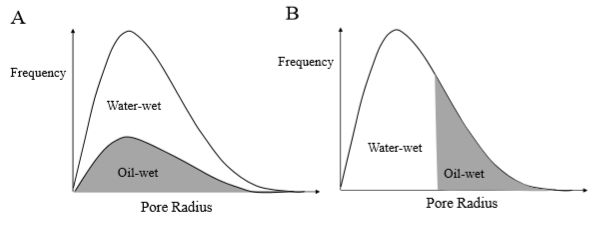
\includegraphics[width=1\textwidth]{\dir/figs/wetsystem}
  \caption{Two wetting systems. For a fractionally-wet system (A), bot oil-wet and water wet pores can both be found in all range of pore radius. For a mixed-wet system (B), water-wet pores and oil-wet pores are separated by a threshold pore radius. Image adapted from \citet{mcdougall1995impact}}
  \label{wetsystem}
\end{figure}

\paragraph{Contact angle hysteresis}
For a stationary fluid droplet on a surface, the contact angle is fixed. However when the fluid droplet is in motion, the contact angle will have different values depending on the direction of motion and wettability. Shown in Fig.\ref{anglehyster}, when the wetting fluid is receding, the receding contact angle $\theta_R$ (1) will decrease compared with the contact angle in equilibrium $\theta_E$ (2). When the wetting phase is advancing, the advancing contact angle $\theta_A$ (3) will increase  compared with $\theta_E$. The difference between advancing and receding contact angles is known as contact angle hysteresis \citep{gao2006contact}. For non-wetting invasion, the displacement is limited by the smallest effective contact angle, the receding angle $\theta_R$. For wetting invasion, the displacement is limited by the largest effective contact angle, the advancing angle $\theta_A$. A pragmatic consequence of contact angle hysteresis is that, when measuring the contact angle (assuming the wetting phase is the denser phase so the contact angle is measured with regard to the wetting phase), the apparent contact angle measured when the fluids are in equilibrium is close to the true contact angle. The contact angle measured during drainage in motion is larger than the true contact angle. The contact angle measured during imbibition in motion is smaller than the true contact angle. There are four reasons for contact angle hysteresis \citep{blunt2017multiphase}: 1) Wettability alteration 2) surface roughness 3) chemical heterogeneity and 4) flow rate.

One pragmatic consequence of the contact angle hysteresis is that, in fast synchrotron experiments which temporal resolution can be around a second, the x-ray imaging may capture both fluid in motion as well as fluid in stagnation. When measuring the contact angles based on such x-ray images, part of the measurements that taken on moving parts of the fluid can be less accurate due to contact angle hysteresis. 

\begin{figure}[htbp]
  \centering
  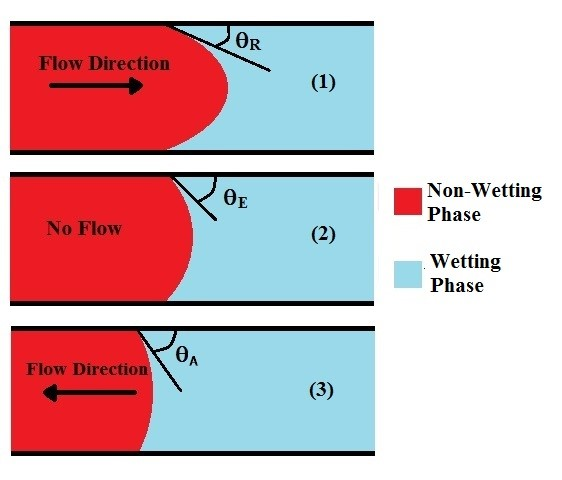
\includegraphics[width=0.7\textwidth]{\dir/figs/anglehyster}
  \caption{Contact angle hysteresis. For contact angle measured in the non-wetting phase (red), the receding contact angle $\theta_R$ that measured at the advancing front is smaller than the genuine contact angle measured at fluid equilibrium $\theta_E$. The advancing contact angle $\theta_A$ that measured on the rear of a moving fluid body is greater than $\theta_E$. Image adapted from \citet{kantzas2012fundamentals}.}
  \label{anglehyster}
\end{figure}

\subsubsection{Wettability alteration}
The wettability of major rock-forming minerals in sedimentary rocks, such as calcite and quartz, is naturally water-wet \citep{abdallah1986fundamentals}. Therefore sedimentary rocks such as sandstone and carbonates, are predominantly water-wet prior to oil migration. However, the wettability of a rock surface can be altered naturally by geological process, due to the deposition of heavy and polar components of the crude oil, such as asphaltenes and resins, on the rock surface. These polar molecules, either acidic-charged or basic-charged \citep{benner1941effect}, can interact with the surface of minerals exposed on the rock surface and therefore alter the wettability in contact \citep{crocker1988wettability}. For core-flooding experiments in the context of oil recovery, it is crucial to conduct experiments in mimic reservoir conditions, including temperature, pressure and wettability. So a process called aging is adopted to artificially alter the wettability of a "clean" rock sample to simulate the wettability condition in reservoir. Aging is a crucial method in core analysis studies and has been increasingly used and discussed in related studies \cite{anderson1986wettability,al2005wettability,kowalewski2003wettability}. 
\paragraph{Wettability alteration in reservoir}
For a typical oil reservoir, the reservoir rock was saturated with an aqueous phase - reservoir brine prior to oil migration. When oil migrated into the reservoir, it entered as the non-wetting phase, while the brine stayed close to the rock surface. As oil migration proceeded, oil replaced the brine in place and left behind an irreducible brine saturation. The residual brine, as the wetting fluid, resided as thin brine films coating the rock surface, and resided as thin layers in the corners, throats, roughness and narrow crevices of the pore space, while oil occupying the pore centres. Crude oil can alter the adjacent rock surface in two ways: by diffusion of polar molecules through the brine film \citep{cuiec1984rock,anderson1986wettability}, or by direct reaction with the surface by brine film collapse \citep{hirasaki1991wettability,buckley1996mechanisms}.

As in one single pore both wetting and non-wetting fluid can co-exist because of the crevices that allow wetting fluid to persist, and different fluid configuration in a single pore can result in different wettability alteration patterns in that pore. \citet{kovscek1993pore} discussed two phase fluid configuration in star-shaped pore and the wettability pattern. \citet{hui2000effects} discussed three phase fluid configuration in triangle-shaped pore and the wettability pattern. These discussions are very important because the wettability alteration in a single pore is non-uniform due to the existence of brine film and wetting corners. This results in non-uniform wettability of single pore \ref{wetconfig}:

\begin{figure}[htbp]
  \centering
  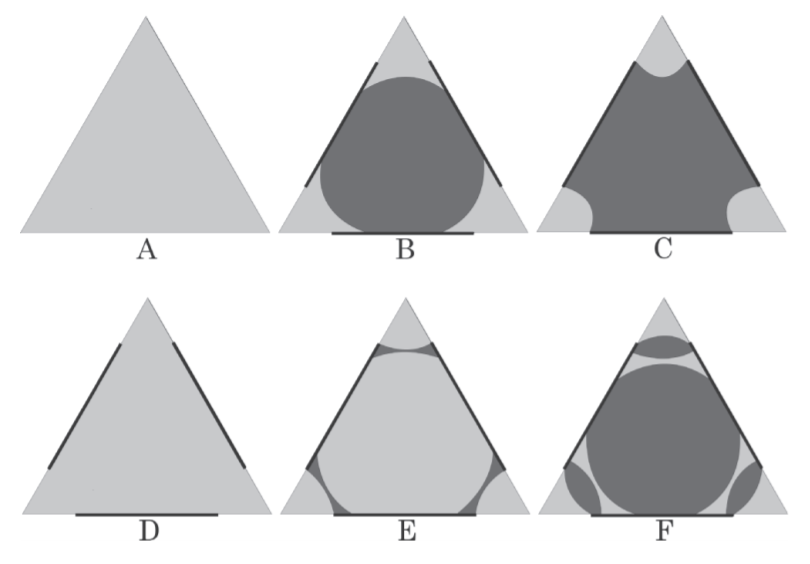
\includegraphics[width=1\textwidth]{\dir/figs/wettabilityconfig}
  \caption{Possible fluid configurations for water (blue) and oil (red) in wettability-altered triangle-shaped pore cross-section. Bold line indicates altered surface wettability. A: water-wet unaltered pore. B: pore body altered to less water-wet. C: pore body altered to oil-wet. D: pore body altered but still strongly water wet. E: Oil only exist as thin layer between corner flow and main water body, therefore only the contacting surface became oil-wet. F: the combination of B and E, but the contacting surface altered to only slightly water-wet. Modified from \citet{helland2006physically}}
  \label{wetconfig}
\end{figure}

\paragraph{Wettability alteration in laboratory}
In the laboratory the aim of wettability alteration is to establish wettability condition that resembles the reservoir \citep{al2005wettability}, because it is one of the major controlling factor of fluid flow. To achieve this, aging is conducted at simulated reservoir condition, including temperature, pressure, connate brine saturation and composition and crude composition. 

The initial step of aging is saturating the cleaned sample core plug with brine. Then crude oil is introduced into the porosity by injection or centrifugation to replace the brine until representative initial water saturation is achieved. The residual brine is assumed to form thin films that has two crucial impacts, first determine the pattern of wettability alteration inside the pores, second take part and assist in the aging process \citep{buckley1996mechanisms}. The aging process lasts for many weeks at reservoir temperature and pressure.

\citet{Pak2014thesis} reviewed a number of studies that identified the main controlling factors for wettability alteration. The main factors are 1) crude oil chemical composition, 2) mineralogy (surface charge) of the rock, 3) salinity and composition of the brine and 4) aging time and temperature. The factors are listed as an overview but will not further discussed because they are beyond the scope of this thesis.


\subsection{Capillary pressure}
When two fluids present in a porous medium, each fluid exerts pressure at the interface of the two fluids. The difference in pressure of the two fluids at the fluid interface is defined as local capillary pressure.

The simplest demonstration of capillary pressure is the capillary rise experiment \citep{young1805iii,leverett1941capillary} in which capillary pressure can be directly visualised. In a capillary rise experiment, the porous medium is of its simplest form - cylindrical tube(s). And the fluids are usually liquid (water, mercury) and gas (air).

Figure \ref{capillaryrise} shows a conceptual illustration of a capillary rise experiment. For a water-air system (a), water is the wetting fluid, the capillary pressure on the fluid interface works against the atmospheric pressure and gravitational force, resulting in a rise of water column by distance $h$ in the tube. For a mercury-air system (b), air is the wetting fluid. The net effect of capillary pressure, atmospheric pressure and gravitational force is a drop of mercury in the tube. 

For a cylindrical tube of diameter $d$, with two fluids of contact angle \texttheta. Given the interfacial tension \textsigma of the two fluids, capillary pressure at the fluid interface can be calculated using the below equation:

\begin{equation}\label{pc}
    P_c=\frac{2\sigma cos \theta}{r}
\end{equation}

This equation stated that, for a interface of two given fluids (thus fixed \textsigma) at a cylindrical pore throat, the local capillary pressure is proportional to the contact angle, and inversely proportional to the radius of the throat. This equation is derived from the fundamental Young-Laplace equation which will be discussed in the following section. The equation \ref{pc} also explains the fact that in a porous medium, the wetting fluid tends to first occupy pores and throats of the smallest diameter, then fill larger pores in the order of ascending diameter. It is vice versa for non-wetting fluid, which tends to first occupy the largest pores, and then fill smaller pores in the order of descending diameter.

\begin{figure}[htbp]
  \centering
  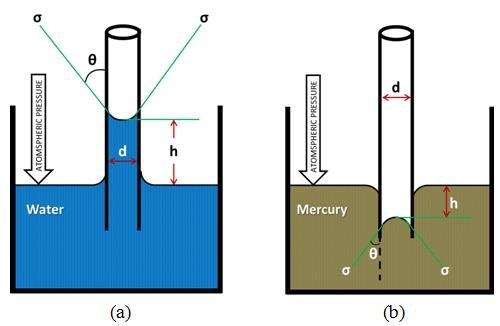
\includegraphics[width=1\textwidth]{\dir/figs/Capillaryrise}
  \caption{Conceptual capillary rise experiment. The tube (diameter $d$) is water-wet, when the tube is immersed in water (a), the vertical component of the capillary force ($\sigma$) works against atmospheric pressure and gravity, caused a rise $h$ of the water body. When the fluid is mercury (b), the contact angle caused the capillary force pointing $\sigma$ downwards. the vertical component of $\sigma$ work along with atmospheric pressure and gravity, caused a drop $h$ of the mercury body. Adapt from \citet{kerimov2014middle}.}
  \label{capillaryrise}
\end{figure}

The fundamental difference of capillary pressure of the wetting and non-wetting fluids categorises fluid flow into two domains: imbibition and drainage. Imbibition refers to the process of a wetting-fluid displacing a non-wetting fluid, and drainage refers to the process of a non-wetting fluid displacing a wetting fluid (Fig.\ref{drainandimbib}). The term imbibition can be easily conceptualised as the process of imbibe water (or any other wetting fluids) in a water-wet medium, and drainage as the process of drain the water by air (or any other non-wetting fluids).

\begin{figure}[htbp]
  \centering
  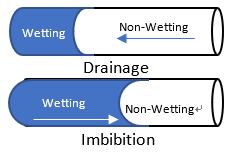
\includegraphics[width=0.7\textwidth]{\dir/figs/drainandimbib}
  \caption{Drainage and imbibition. Drainage is the process of non-wetting fluid displacing wetting fluid. Imbibition is wetting fluid displacing non-wetting fluid}
  \label{drainandimbib}
\end{figure}

\subsection{Drainage}
For a porous medium containing two immiscible fluids, the capillary pressure increases where the pore radius decreases. This means when fluids flow in a porous medium there is a pressure gradient. Fluids flow from high pressure to low pressure, so in drainage process, it is the narrowest restrictions that limit the non-wetting fluid movement.

\subsubsection{Primary drainage}
As mentioned before, the majority of natural rocks are water-wet prior to oil migration, and is entirely saturated with the wetting phase. The first time a non-wetting phase enters the system, this is a primary drainage process. Some common examples of primary drainage in natural systems are \citep{blunt2017multiphase}: the migration of hydrocarbons (liquid or gas) from source rock to a reservoir, the injection of $CO_2$ into a saline aquifer and the process of mercury injection capillary pressure (MICP) for the measurement of pore-size distribution.

During drainage, to enter a pore, the non-wetting fluid must overcome the threshold capillary pressure governed by the locally smallest throat radius $r_t$. The interface between the moving front of the non-wetting fluid and the receding non-wetting phase is called a terminal meniscus (TM) shown in Fig.\ref{tm}. The terminal meniscus can be experimentally identified observed by a distinctive curvature distribution \citep{andrew2015imaging}.

\begin{figure}[htbp]
  \centering
  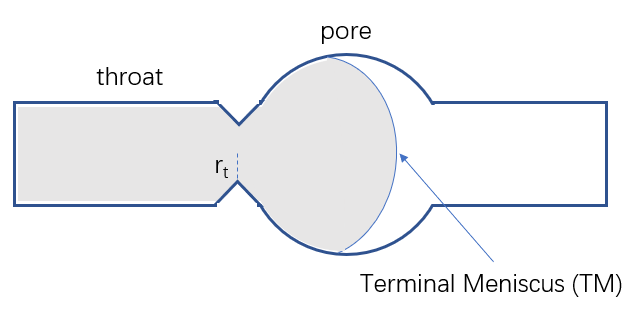
\includegraphics[width=0.6\textwidth]{\dir/figs/tm}
  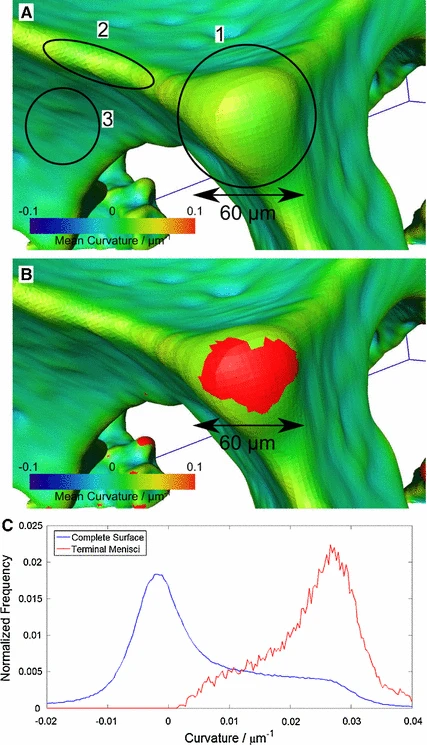
\includegraphics[width=0.6\textwidth]{\dir/figs/terminalmeniscus}
  \caption{Terminal meniscus. The uppermost figure shows the terminal meniscus span across the widest place of a pore in 2D section. The next three figures (A,B,C) are adapted from \citet{andrew2015imaging}. A shows 3D visualisation of a terminal meniscus (circle 1) formed by the fluid (green). B shows curvature measurement on the fluid surface mesh. C shows distinct curvature distribution of the terminal meniscus and the complete surface.}
  \label{tm}
\end{figure}

\subsubsection{Wetting layers}
During drainage, the non-wetting fluid movement is impeded by the narrowest pore throats. Since the pore geometry in a real rock is highly irregular, the wetting phase can reside in the crevices and corners of the pore space. These narrow regions have very high capillary entry pressure thus the wetting fluid inside can not be removed by the non-wetting fluid. These retained wetting fluid can be widely connected throughout the pore network, and are known as wetting layers. Wetting layers are experimentally verified both in 2D and 3D \citep{datta2014mobilization, andrew2015imaging}. Wetting layers have different flow properties than wetting films \citep{blunt2017multiphase}. Wetting films cover the surface of the solid, their thickness is molecular-scale and does not support significant fluid flow. In contrast, wetting layers that reside in the crevices and corners are of macroscopic (few microns) thickness and therefore allow appreciable flow movement.

\begin{figure}[htbp]
  \centering
  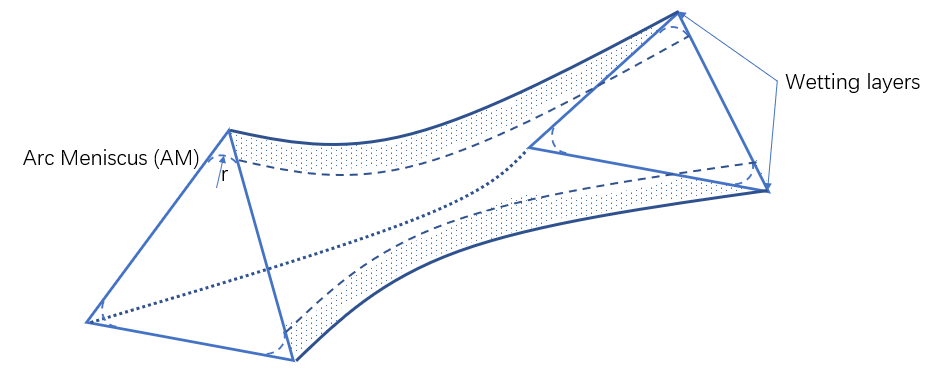
\includegraphics[width=0.9\textwidth]{\dir/figs/wl}
  \caption{Wetting layers and arc meniscus. For a pore system with corners (simplified as a triangle-shaped cross section), thus allowing corner flow, wetting layers can exist in the corners and connect throughout many pores in the system. The curvature (radius $r$) of the wetting layer forms the arc meniscus. Redrawn from \citet{blunt2017multiphase}}
  \label{wl}
\end{figure}

Fig.\ref{wl} demonstrates the conceptual fluid configuration of wetting layers in a simplified pore throat. The wetting layers are crucial structures for fluid flow in porous media, because they allow wetting fluid flow throughout the pore network even at high non-wetting saturation, and allow the important mechanism of snap-off to occur during imbibition.

\subsubsection{Haines jumps}
During drainage, the non-wetting fluid will retract from regions of high pressure and move towards low pressure following the pressure gradient. The local pressure gradient leads to a rapid filling, regardless of the slowness of external rate of injection, of a series of wider pores in order to achieve capillary equilibrium. Meanwhile, the non-wetting fluid retracts from regions of high pressure to allow the filling of low pressure regions.

This process of fluid rapidly filling multiple pores is called Haines jumps \citep{haines1930studies}, firstly discovered in soil moisture studies. Different from the gradual filling of a pore which can be filled by a smooth reversible process, Haines jumps are quantised, meaning that the pores are filled by Haines jumps by an irreversible, instantaneous process. Capillary equilibrium can only be established before and after the jumps, but the jump process is unstable, therefore there is no half-filled pore by Haines jumps.

In the core flooding experiments by \citet{berg2013real}, they correlated small pore pressure fluctuations with multiple fast pore filling events seen before and after in scans. The finding changed the common singular pore jump paradigm of Haines jumps. One Haines jump typically cascade through 10-20 geometrically defined pores. Fig.\ref{hj} shows Haines jump events of different scale imaged by synchrotron microtomography \citep{berg2013real}. The upper row of images shows a large scale Haines jump event that affected several connected pores. The bottom row shows a small scale Haines jump event that filled single pore. These events were proved genuine by pressure records.

\begin{figure}[htbp]
  \centering
  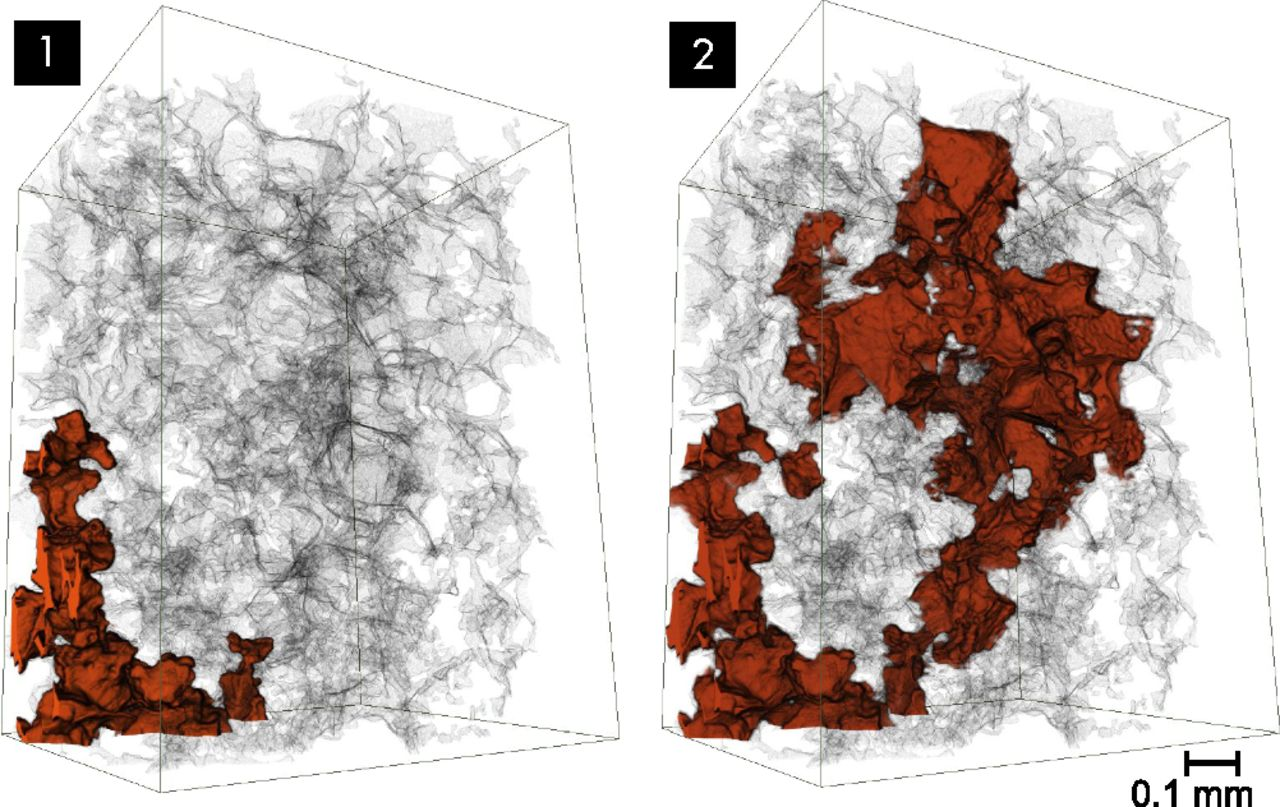
\includegraphics[width=0.9\textwidth]{\dir/figs/hjlarge}
  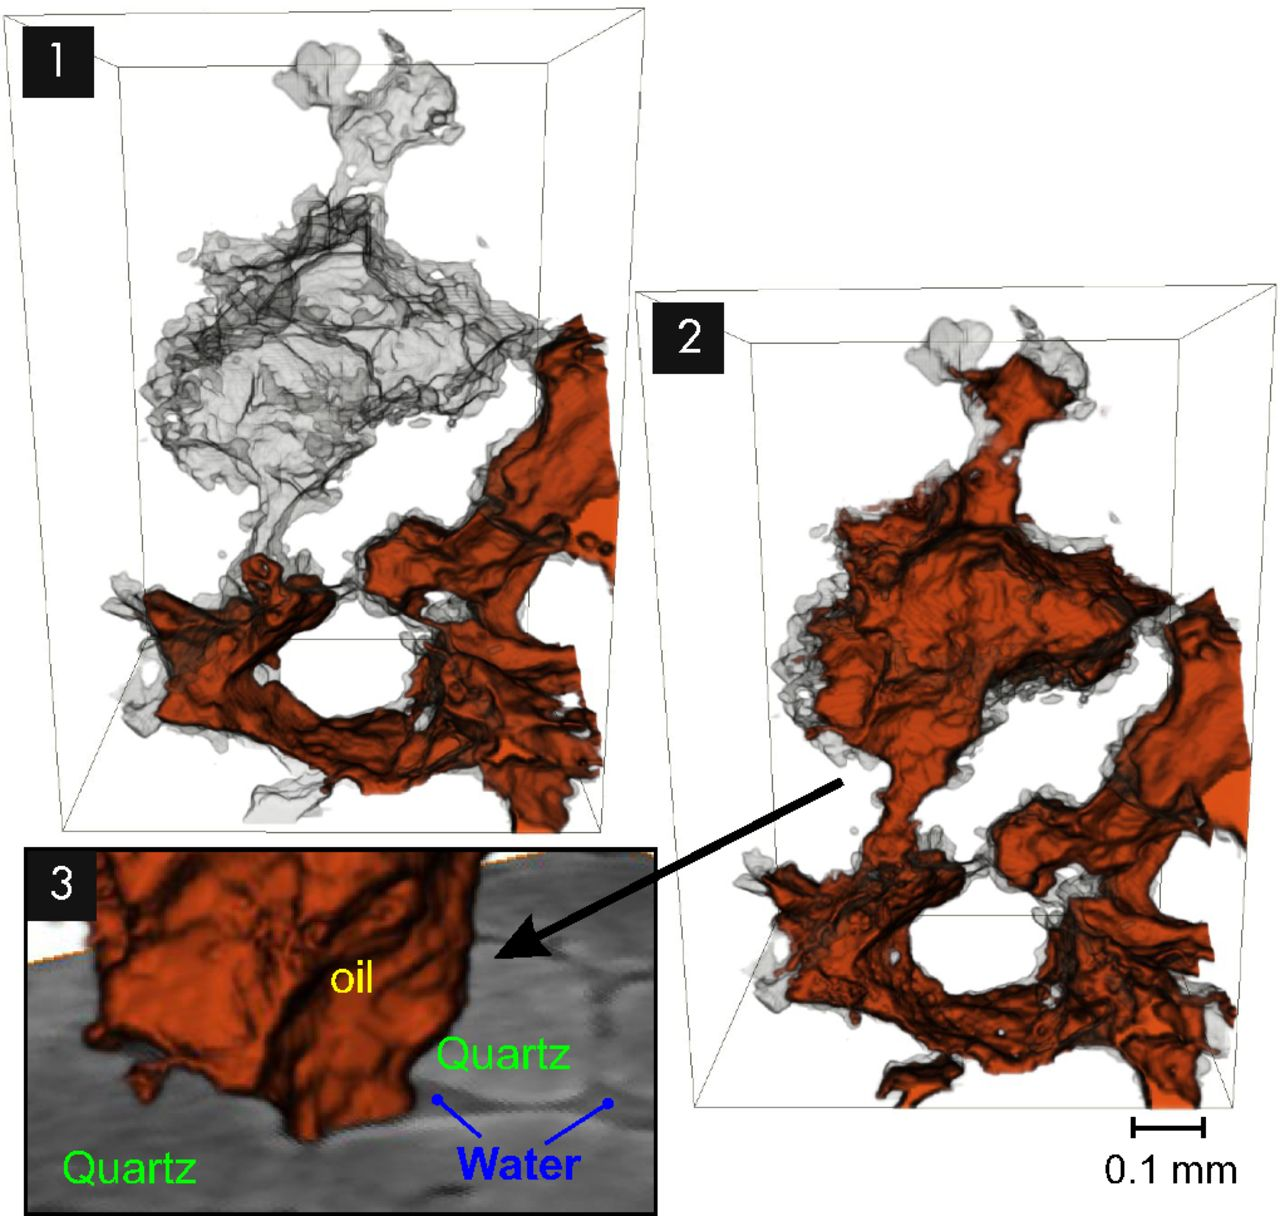
\includegraphics[width=0.9\textwidth]{\dir/figs/hjsmall}
  \caption{Haines jumps of different scales. The upper two images shows a large scale Haines jump (timestamp 1-2) of oil that span across 10+ pores. The lower three images shows a small scale Haines jump (timestamp 1-2) that only affect one pore. 3 is the zoomed-in image that shows the oil, water and rock phase corresponding to the 2D CT reconstruction image. Adapt from \citet{berg2013real}.}
  \label{hj}
\end{figure}

A Haines-jump event involves fast filling of multiple pores, and consequently the retraction and snap-off of the non-wetting phase at higher-pressure regions. Importantly, the retraction of non-wetting phase can be non-local, i.e. can occur throughout the system. Such retraction is a local imbibition process in a drainage event. \citet{andrew2015imaging} imaged a Haines-jump event of super-critical $CO_2$ displacing brine in Ketton limestone during primary drainage. The captured Haines-jump event resulted in the retraction and snap-off of the non-wetting phase that is distal and indirectly involved with the Haines-jump event (Fig.\ref{distalretraction}).

\begin{figure}[htbp]
  \centering
  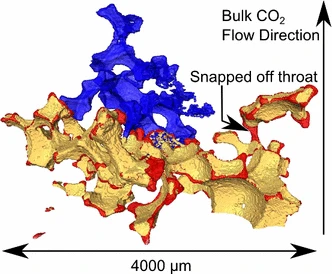
\includegraphics[width=0.75\textwidth]{\dir/figs/distalretraction}
  \caption{Haines jump can cause retraction of the non-wetting fluid, even at a distance from the pore where Haines jump occurs. Yellow is the non-wetting fluid $CO_2$. Blue is the Haines jump event. Red shows the retraction of $CO_2$ after the Haines jump event. A distal snap-off event (notation with arrow) happened few pores away from the Haines jump event. Image adapt from \citet{andrew2015imaging}.}
  \label{distalretraction}
\end{figure}

\subsubsection{Roof snap-off}
Haines jumps are associated with one important mechanism called Roof snap-off. It is a phenomenon that when non-wetting fluid emerge from a throat into a pore, the capillary pressure is in favour of separating the leading portion of the non-wetting fluid into droplets (Roof snap-off), and rapidly fill the adjacent pore in an irreversible Haines jump-fashion. Roof snap-off is firstly directly observed by \citet{roof1970snap} during drainage in an idealised pore geometry. A simplified diagram of a Roof snap-off event is shown in Fig.\ref{roofdemo}.

In Fig.\ref{roofdemo} upper figure, shows the critical radius of the terminal meniscus $r_{crit}$ being reached by the invading non-wetting fluid. This is the critical onset moment of a Roof snap-off event. After the critical radius of the $r_{crit}$ has been reached (middle figure), the surface tension is in favour of splitting the moving front of the non-wetting fluid into a droplet. This is the ongoing moment of a Roof snap-off event, while snap-off in imbibition requires thickening of wetting layers, Roof-snap off can occur without wetting layers but through thin film flow \citep{roof1970snap, gauglitz1990dynamics}. The fluid interface will rapidly recover to the smallest to minimise the surface energy. The Roof snap-off can happen several times, rapidly, until the adjacent pore is completely filled by the non-wetting phase (bottom figure). The non-wetting fluid in the throat will retract and form new terminal meniscus with a radius of curvature $r$. The new capillary equilibrium will be lower than pre-snap-off, indicated by $r>r_{crit}$. At the end of the event, the pore is end with a trapped non-wetting ganglion (blob) in the pore space (bottom figure). The trapped ganglion can be reconnected once the throat filled by more incoming non-wetting fluid.

\begin{figure}[htbp]
  \centering
  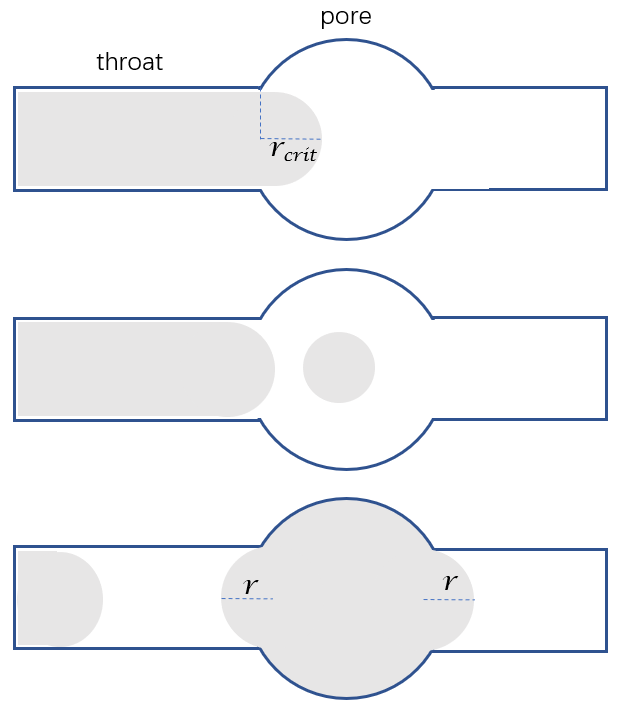
\includegraphics[width=0.7\textwidth]{\dir/figs/roofdemo}
  \caption{Conceptual Roof snap-off in a 2D pore section. The top figure shows the onset of a Roof snap-off event, the non-wetting fluid enters the pore and reached a critical radius $r_{crit}$. The middle figure shows the ongoing Roof snap-off that the front of the non-wetting fluid is snapped-off. The bottom figure shows that once the snap-off began, the pore will be rapidly filled by repeating snap-off. The new equilibrium is reached when the pore is completely filled, and disconnected with its feeding body.}
  \label{roofdemo}
\end{figure}

\subsection{Imbibition}
Imbibition is the reverse process to drainage, i.e. the process of a wetting fluid displacing the non wetting fluid. Capillary pressure by definition is the difference of non-wetting and wetting phase. During imbibition the wetting fluid saturation is increased therefore the capillary pressure in the system is decreased. 

Imbibition examples in nature can be soaking of water into soil and absorption of water into dry woods etc. The first entry of the wetting fluid into a porous medium is primary imbibition, for example the filling of dry sand by water. After primary drainage, the pore space is mostly saturated with non-wetting phase, but wetting phase can still exist in the form of wetting films and wetting layers. In this case, the re-entry of wetting fluid is secondary imbibition \citep{blunt2017multiphase}. The example of secondary imbibition can be water-flooding an oil reservoir (if the reservoir rock is water-wet).

There are two type of processes that occur during imbibition: snap-off and piston-like advance. The imbibition process is ultimately controlled by the competition of snap-off and piston-like advance (Fig.\ref{pistonandsnappoff}). These two important processes will be introduced in the following sections.

\begin{figure}[htbp]
  \centering
  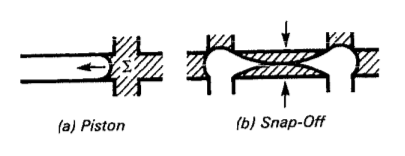
\includegraphics[width=1\textwidth]{\dir/figs/pistonandsnapoff}
  \caption{Two major filling mechanisms in imbibition. (a) Piston-like advance which wetting fluid displacing non-wetting fluid in a piston-like motion. (b) Snap off, wetting films can bulge or swell and eventually merge to fill a previously non-wetting occupied throat. Adapt from \citet{lenormand1984role}.}
  \label{pistonandsnappoff}
\end{figure}

\subsubsection{Piston-like advance}
Piston-like advance is the direct filling of pore space by wetting fluid. Wetting fluid during piston-like advance has a rather flat front and leaves very little non-wetting fluid trapped behind (Fig.\ref{pistonandsnappoff} (a)). The presence of wetting layers is crucial for spontaneous filling of the wetting phase in piston-like advance, it is theoretically proven that the wetting layers make the throat appear more water-wet than without them \citep{ma1996effect,oren1998extending}.

\subsubsection{Cooperative pore filling}
During imbibition the capillary pressure is always decreased, therefore the wetting fluid will preferentially fill throats rather than pores. That is to say, in contrast with drainage that is impeded by throats, the imbibition process is impeded by pores. The pore filling criterion for imbibition is governed by capillary entry pressure which is decided by the largest curvature radius of the terminal meniscus. To decide the critical curvature radius in one particular pore, we have to not only consider the size and shape of the pore, but also consider the wetting fluid saturation of the bounding throats of that pore. If the filling of a pore is assisted by wetting fluid in the bounding throats, then this is cooperative pore filling in imbibition.

Firstly discussed by \citet{lenormand1983mechanisms,  lenormand1984role}, the cooperative pore filling mechanism is named $I_n$, where n is the number of bounding throats that filled by non-wetting fluid. For example if a pore has one adjacent throat that filled by non-wetting fluid, this is an $I_1$ cooperative pore filling process.

\begin{figure}[htbp]
  \centering
  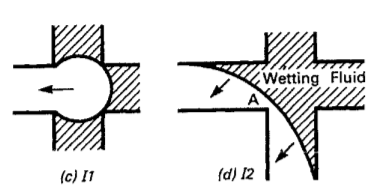
\includegraphics[width=1\textwidth]{\dir/figs/i1i2}
  \caption{Cooperative pore filling event $I_1$ and $I_2$. $I_1$ shows when only one adjacent throat is filled by non-wetting fluid. $I_2$ is when two of the adjacent throats are filled by non-wetting fluid. The critical radius of the curvature $I_1$ is smaller than $I_2$ therefore an $I_1$ event is more preferred to happen than $I_2$ while both events are possible. Adapt from \citet{lenormand1984role}.}
  \label{i1i2}
\end{figure}

First we look at an $I_1$ process (Fig.\ref{i1i2} left). This denotes an $I_1$ process because the pore has only one adjacent throat that is filled by non-wetting fluid. The largest curvature radius of the terminal meniscus is the radius of the circle in the middle which is also the pore radius. An $I_2$ process (Fig.\ref{i1i2} right) is where two of the adjacent throats are filled by non-wetting fluid. I2 has much larger curvature radius of the TM, thus is less favoured by the wetting fluid. 

$I_3$ and higher $n$ processes are rarely seen \citep{blunt2017multiphase}, and it is theoretically demonstrated that higher $n$ events are less favoured by the imbibition process \citep{blunt1998physically,oren1998extending}. A simulation was done in a Bentheimer sandstone pore network model to quantify the frequency of events in imbibition \citep{blunt2017multiphase}, and the result agreed with the theoretical implication that higher $n$ events are less frequent.

One important feature of cooperative pore filling in imbibition is that theoretically it leads to a flat frontal advance with no trapping \citep{blunt1992simulation}. In the simulation the wetting phase displaced the non-wetting phase by a cycle of $I_3$ - $I_2$ events therefore leading to a flat frontal advance with no trapping (Fig.\ref{frontadvance}.

\begin{figure}[htbp]
  \centering
  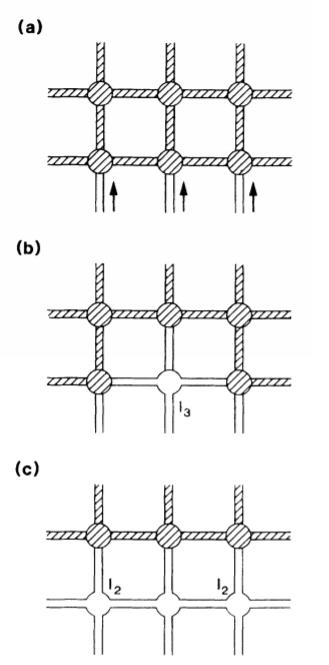
\includegraphics[width=0.5\textwidth]{\dir/figs/frontaladvance}
  \caption{Flat frontal advance associated with cooperative pore filling in imbibition, in a pore system with relatively homogeneous pore size distribution. Dashed line stands for non-wetting fluid and blank stands for wetting fluid. Arrow is the direction of the flow. (a) shows three pores that are all potentially $I_3$ filling events, chances are equal that one of the pore can be filled by an $I_3$ event. (b) When one of the pore is filled by an $I_3$ event, the filling of the rest two pores became two potential $I_2$ events. Because $I_2$ is more preferable than $I_3$, the rest two pores will be filled rather than going for another $I_3$ event. (c) When the rest two pores were filled by two $I_2$ events, it becomes the same situation as (a) where three potential pores are all $I_3$ events. This filling cycle will lead to a flat frontal advance with no trapping left behind. Image adapt from \citet{blunt1992simulation}.}
  \label{frontadvance}
\end{figure}

\subsubsection{Wetting layer swelling and snap-off}
In imbibition, the swelling of wetting layers leads to snap-off (Fig.\ref{pistonandsnappoff} (b)). Snap-off was first described by \citet{pickell1966application}. It occurs in the narrowest region of the throats, leading to partial filling of the two adjacent pores. A demonstration of the wetting layer swelling and snap-off is drawn as Fig.\ref{snapoffdemo}.

During imbibition, the wetting phase can flow in the wetting layers and therefore increase their thickness. Before a snap-off event, the wetting layers keep swelling until they meet. The swelled wetting layers are most easily met at the narrowest region of the throat, and this is when snap-off begins. Two terminal menisci that curved towards opposite direction are formed where the wetting layers met. The entire throat will be rapidly filled by the wetting fluid once snap-off occurs, consequently the two terminal menisci will retreat to a critical radius that allows new capillary equilibrium to establish.

\begin{figure}[htbp]
  \centering
  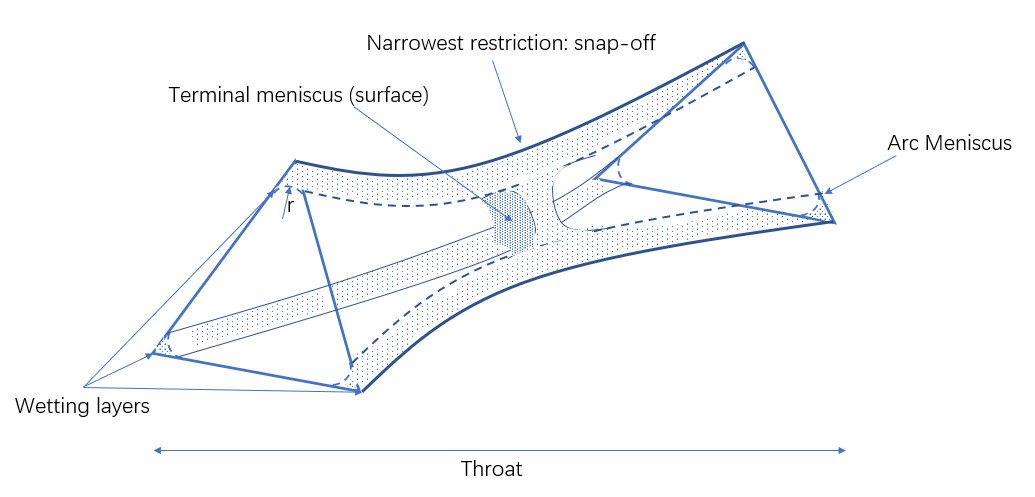
\includegraphics[width=1\textwidth]{\dir/figs/snapoffdemo}
  \caption{Snap-off illustrated in a simplified throat. The wetting layers allows wetting fluids flow in corners and crevices while non-wetting fluid occupying the centre of the throat. During imbibition, wetting layers can swell and easily merge at the narrowest point of the throat, causing snap-off of the existing non-wetting fluid and eventually fill the entire throat. Redrawn from \citet{blunt2017multiphase}}
  \label{snapoffdemo}
\end{figure}

\subsubsection{Displacement patterns in imbibition}
The competition between snap-off and piston-like advance forms four generic types of displacement patterns in imbibition \citep{chandler1982capillary,lenormand1984role,cieplak1988dynamical,cieplak1990influence}: 1) percolation with trapping, 2) invasion percolation, 3) frontal advance and 4) cluster growth. The term percolation comes from the approach of representing a porous medium using a network model. The pores and throats were analogous to 'sites' and 'bonds' of a percolation process \citep{broadbent1957percolation}.

The first type of pattern is percolation with trapping. In a heterogeneous porous medium that allows flow in wetting layers, pores and throats are filled in order of size. Flow in wetting layers are connected throughout the pore system so that imbibition can take place anywhere in the system. Non-wetting phase can be trapped by snap-off events. This is the most commonly encountered case in reservoir settings \citep{blunt2017multiphase}.

The second type invasion percolation is similar to the first type, but without flow in wetting layers (for example primary imbibition into a dry rock). This results in limited choice of pore-filling that does not purely dependent on order of size, but also the accessibility of fluids. 

The third type flat frontal advance is more common in less heterogeneous medium, where cooperative pore-filling is in dominance. The advancing front of the wetting fluid is flat due to the repetition of $I_n$ processes (Fig.\ref{frontadvance}. Non-wetting fluid is rarely trapped. An example of this type of displacement is paper towel soaking water. 

Cluster growth is similar wit frontal advance, but crevice flow exists. Wetting layers allow fluid to access any pore in the system, therefore pore-filling can happen distance away from inlet. Instead of flat frontal advance from the inlet, in this type of imbibition pores are filled as growing clusters inside the porous medium and left almost no trapped non-wetting phase. This type could occur in a pore system where the pores and throats are of similar size \citep{blunt2017multiphase}.

\subsection{Relative permeability}
\paragraph{Relative permeability definition}
The permeability introduced at the beginning of this section is also known as absolute permeability, and is only valid for a porous medium that is completely saturated by the measured flowing fluid \citep{honarpour2018relative}. For immiscible multiphase fluid flow, the more useful representation of permeability is effective permeability which for each fluid is a function of its percentage saturation.

Relative permeability is defined as the dimensionless ratio of effective permeability to absolute permeability. For two phase flow of oil and water, the relative permeability of oil and water is noted as $k_{ro}$ and $k_{rw}$ respectively. The general shape of $k_{ro}$ and $k_rw$ can be approximately represented by $k_{rw}=A(S_w)^n$, $k_{ro}=B(1-S_w)^m$ where $S_w$ is the saturation of water and A,B,m,n are constants.

\paragraph{Relative permeability during drainage and imbibition}
Assuming a water-wet porous rock that initially saturated with 100\% water. At this time $k_{rw}=1$ and $k_{ro}=0$. During primary drainage, the oil first traverses through the largest pores, resulted in disconnecting the most conductive paths (narrow throats) for water therefore $k_{rw}$ drops rapidly. Meanwhile as oil saturation increases and more oil pathways are established, $k_{ro}$ will rise. $k_{ro}$ and $k_{rw}$ curves will eventually cross as drainage continues, the water saturation of the crossing point will vary in different rocks. Because the increase of $k_{ro}$ and the decrease of $k_{rw}$ follow a power law, the relative permeability for both fluids at the crossing point is much less than 0.5, and so the sum of the relative permeabilities of the two fluids is then much less than 1. This means that the total flow of both fluids are impeded \citep{blunt2017multiphase}.

At some point when the oil saturation is high enough for oil to become well connected, the $k_{ro}$ will rise sharply approaching 1. At this time water has reached an irreducible saturation and only exists in form of wetting layers and wetting films. $S_w$ and $k_{rw}$ approach a very low value. 

Relative permeability during secondary imbibition is not the reverse process of primary drainage, because for that the non-wetting phase can be trapped by snap-off events. During secondary imbibition snap-off can disconnect oil pathways with little change in water saturation, leading to a sharp drop of $k_{ro}$ \citep{blunt2017multiphase}. The irreversibility of $k_{ro}$ is also known as hysteresis. It mainly has two causes \citep{spiteri2005relative} 1) contact angle hysteresis. In imbibition there are three ways for water to displace oil: piston-like advance, snap-off and cooperative filling. All three displacement mechanisms are strongly dependent on the wettability, therefore the contact angle hysteresis that changes the intrinsic contact angle to the advancing contact angle leads to change in apparent wettability and resulted in change in displacement mechanism, and ultimately leads to relative permeability hysteresis. 2) trapping of the non-wetting phase. Once the non-wetting phase is trapped by snap-off events, $k_{ro}$ will have a significant drop due to disconnected oil path, and consequently causes relative permeability hysteresis.

The relative permeability of water $k_{rw}$ does not have hysteresis \citep{blunt2017multiphase}. For that water can not be completely trapped therefore has similar conductance for similar saturation, regardless of the displacement process. 

\subsection{Capillary number and flow regime}
Permeability, as previously discussed, is an intrinsic property that as a function only of the pore geometry. This is under the assumption that while a fluid is moving, its velocity field does not change with time. However when the flow rate is high that viscous forces (the friction inside a fluid) become significant enough to cause changes to the velocity field, it consequently alters the microscopic configuration of fluid. Furthermore, it makes relative permeability dependent on Darcy velocity, and challenges the inherent assumption of the multiphase extension of Darcy's law \citep{blunt2017multiphase}. Therefore the impact of flow rate needs to be discussed in order to characterise flow in porous medium. First of all, rather than treating viscous forces and capillary forces separately, a dimensionless capillary number $Ca$ is introduced to represent the net effect of viscous forces and capillary forces between two immiscible fluids:

\begin{equation}
    Ca= \frac{\mu q}{\sigma}
\end{equation}

where $q$ is the Darcy velocity of the flowing fluid, $\mu$ is its viscosity and $\sigma$ is the interfacial tension between two fluids. However, $Ca$ does not represent the ratio of viscous to capillary effects at pore scale directly, it needs to be multiplied by a geometry-saturation-dependent quantity (much larger than 1) to find the true ratio \citep{blunt2017multiphase}. When $Ca \ll 1$, conventionally $Ca<10^{-6}$ \citep{blunt2017multiphase}, the flow is roughly reckoned as dominated by capillary forces. For $Ca>10^{-6}$, viscous effects are significant enough to perturb the fluid configurations, as contact angle has negligible impact on the flow behaviour. To discuss the impact of flow rate on fluid displacement, a classical micro-model experiment by \citet{lenormand1984role} is taken as an example (Fig.\ref{lenormand}). 

\begin{figure}[htbp]
  \centering
  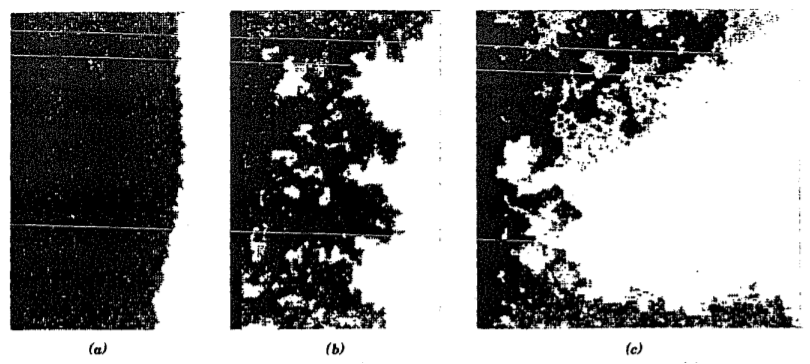
\includegraphics[width=0.8\textwidth]{\dir/figs/lenormand1984}
  \caption{Lenormand's imbibition experiment in a micro model with different flow rate. The micro model contains 42,000 ducts (throats) with 4mm between junctions (pores). The capillary numbers of (a), (b) and (c) are $3\times10^{-4}, 1.4\times10^{-5}$ and $6\times10^{-7}$ respectively. Difference in flow rate caused significant patterns of displacement. At the lowest flow rate, displacement shows flat frontal advance behaviour, and penetrates least of the model length. At the intermediate flow rate, more snap-off and trapping occured. At the highest flow rate, the displacement is the most heterogeneous and penetrates most of the model length, with a percolation-like displacement pattern. Adapt from \citet{lenormand1984role}.}
  \label{lenormand}
\end{figure}

Fig.\ref{lenormand} shows three images of imbibition at different $Ca$. Black is the invading wetting phase injected from left, white is the non-wetting phase being displaced. The $Ca$ from left to right are of $3\times10^{-4}, 1.4\times10^{-5}$ and $6\times10^{-7}$ respectively. Since the interfacial tension and viscosity of a particular fluid stay constant, the only variable is the Darcy velocity, therefore smaller $Ca$ stands for lower flow rate.

At the lowest flow rate (Fig.\ref{lenormand} (c)), where the configuration of fluid at pore scale was controlled by capillary forces only. This is the familiar scenario that have been discussed in the imbibition section. At this rate, the wetting fluid was able to penetrate through most of the model length. The wetting saturation was higher closer to the inlet. There are numerous of isolated non-wetting clusters of non-wetting fluid (white patches inside black) indicating trapped non-wetting fluids. And there shows isolated wetting phase (black patches inside white), indicating the filling of throats by snap-off events, and showing evidence for flow in wetting layers. This is the percolation-like displacement pattern that the pores were filled largely in order of pore size.

At intermediate flow rate (Fig.\ref{lenormand} (b)), the wetting phase travelled shorter of the model length, but the wetting saturation was more homogeneous. There was significantly less snap-off, and trapped non-wetting phase was significantly larger in size.

At the highest flow rate (Fig.\ref{lenormand} (c)), the total volume of trapped wetting phase was low, and confined to small clusters. And there was none snap-off observed. The advancing front was almost flat and the saturation was homogeneous. Piston-like advance was in dominance.

The experiment demonstrates the flow-rate dependency of fluid displacement patterns in imbibition. \citet{blunt2017multiphase}'s interpretation is that, the wetting fluid conductance is low in wetting layers but high through the centres of the pore space. Since layer flow is slow, it has to be sufficiently low flow rate to provide enough time for lots of snap-off events to happen in order of size. If the flow rate is fast, piston-like advance will suppress snap-off events because they can happen much faster. Piston-like advance is more likely to happen near the inlet due to higher wetting fluid pressure. Similar results were also drawn from three dimensional experiments in glass beads packs \citep{datta2014mobilization}.

\subsubsection{Flow regime}
When capillary forces are in dominance, it is possible to describe the multiphase flow using Darcy's law. When viscous forces are in dominance, the inherent assumption of Darcy's law that the displacement pattern is percolation-like is challenged \citep{blunt2017multiphase}. Flow regime refers to the criteria that Darcy's law can or cannot be employed.

A dimensionless number effective capillary number $Ca_{eff}$ is defined as a function of pore length $l$, capillary number $Ca$, porosity $\phi$, permeability $K$ and Bond number $B$ that refers to the ratio of buoyancy to capillary forces:

\begin{equation}
    Ca_{eff}=(\frac{lCa}{\sqrt{\phi K}}+B)
\end{equation}

When viscous forces are in dominance. The flow patterns are controlled by the viscosity ratio $M=\mu_d/ \mu_i$, which is the ratio between the viscosity of the displaced fluid and the injected fluid. $Ca_{eff}$ and $M$ together define the flow regimes\citep{blunt2017multiphase}:

\paragraph{Capillary regime}
When $M<1$ and $Ca_{eff}<1$; or $M>1$ and $Ca_{eff}<1/M$, multiphase Darcy's law is enabled. The flow is capillary-dominated. Displacement pattern is percolation-like.

\paragraph{Viscous regime}
When $Ca_{eff}>1$, the flow is viscous-dominated, and the use of Darcy's law is affected. If $M<1$, the displacement is stable, frontal advance (e.g.Fig.\ref{lenormand} (c)) will occur. If $M>1$, the displacement is unable and will result in viscous fingering, which refers to the onset and evolution of instability during fluid displacement \citep{homsy1987viscous}. For the extreme when $M \rightarrow \infty$, flow pattern is fractal, called diffusion limited aggregation (DLA \citep{witten1981diffusion}).

\subsection{The Young-Laplace equation and Navier-Stokes equation}
For a system of a porous medium containing two immiscible fluid phases, the flow process in this system is ultimately governed by the conservation of three physical properties: the conservation of interfacial energy between fluids, the conservation of momentum and the conservation of mass \citep{blunt2017multiphase}. The two fundamental equations that describe fluid flow in a porous system, namely the Young-Laplace equation and Navier-stocks equation, are derived from the physical conservations.

\subsubsection{Conservation of energy: the Young-Laplace equation}
Conservation of interfacial energy between fluids, and between fluids and solid, governs the fluid configuration in a pore system at capillary equilibrium, and governs the threshold fluid pressure at which displacement can take place. The conservation of interfacial energy is used to derive the Young-Laplace equation\ref{eqy-l}. 

\begin{equation}\label{eqy-l}
    P_{c}=\sigma(\frac{1}{r_{1}}+\frac{1}{r_{2}})=\kappa \sigma
\end{equation}

where $P_{c}$ (unit $m/Lt^2$, \textpsi ) stands for the local capillary pressure, which is derived from the pressure difference between the non-wetting/wetting fluids $P_{nw}-P_{w}$. $r_{1}$ and $r_{2}$ are the radii of curvature of the two fluids. Interfacial tension, \textsigma, according to definition of \citet{blunt2017multiphase} is \textit{"the energy per unit area of the surface between the phases, or the change in free energy for a change in area $\sigma=dF/dA$"}. $\kappa$ is the total curvature of the interface. The Young-Laplace equation relates the local capillary pressure to a function of the interfacial tension and curvature.

Treating the interfacial tensions as force, when apply a horizontal force balance, the Young equation is obtained:

\begin{equation}\label{eq_young}
    \sigma_{nws}=\sigma_{ws}+\sigma cos \theta
\end{equation}

where $ \sigma_{nws}$ ($N/m$) stands for the interfacial tension between the non-wetting phase and the solid, and $ \sigma_{ws}$ as the interfacial tension between the wetting phase and the solid. The fundamental Young equation is an expression for the relation between contact angle and the interfacial tension between the two fluids and the solid.

This equation involves two important concepts of interfacial tension and contact angle. The contact angle, \texttheta, is the angle of the denser fluid phase between solid and the other phase. Interfacial tension and contact angle will be discussed in detail in the following section.

\subsubsection{Conservation of momentum and mass: the Navier-Stocks equation}
Conservation of momentum leads to the Navier-Stokes equations and their macroscopic counterpart, Darcy's law \citep{darcy1856public}. While conservation of energy deals with stationary state of fluids in capillary equilibrium, conservation of momentum deals with fluids in motion. The Navier-Stokes equation has many forms for different contexts of fluids. For simplicity we consider an incompressible Newtonian fluid of fixed viscosity \textmu , and the Navier-Stokes equation is given as follow \citep{batchelor1967introduction}:

\begin{equation}\label{eq_ns}
    \mu\nabla^{2} \mathbf{v} =\rho(\frac{\partial \mathbf{v}}{\partial t}+\mathbf{v}\cdot \nabla \mathbf{v})+\nabla P -\rho\mathbf{g}
\end{equation}

where $\mu$ is the viscosity of the fluid, $\mathbf{v}$ is the vector velocity field ($\nabla^2$ is the Laplace operator, it measures the divergence of the gradient). The left side term $\mu \nabla^2 \mathbf{v}$ can be interpreted as the difference between the velocity at a point and the mean velocity in a small surrounding volume. The left side of the equation consists of several terms. $\nabla P$ is the pressure gradient that act as the driving force (per volume), and $\rho\mathbf{g}$ is the specific weight of the fluid. The term $\nabla P - \rho\mathbf{g}$ can be interpreted as the driving force for flow. The total acceleration  for a moving fluid is given by $\frac{\partial \mathbf{v}}{\partial t} + \mathbf{v}\cdot \nabla \mathbf{v}$, where $\frac{\partial \mathbf{v}}{\partial t}$ is the local/unsteady acceleration and $\mathbf{v}\cdot \nabla \mathbf{v}$ is the convective acceleration. The equation \ref{eq_ns} is essentially the expression of Newton's second law of motion ($F=ma$) applied to a continuous fluid \citep{blunt2017multiphase}. 

The conservation of mass, and consequently the conservation of fluid volume, leads to the second part of the Navier-Stokes equation for a complete solution for both the fluid pressure and velocity. The conservation of mass considers that for some arbitrary volume of fluid, the rate at which mass crosses its surface equals to the rate of change of mass within the volume. It ultimately derives the following equation:

\begin{equation}\label{eq_mass}
    \nabla \cdot \mathbf{v} = 0
\end{equation}

The physical explanation for Eq.\ref{eq_mass} is that for an incompressible fluid, the velocity field is divergence free.

The Young-Laplace equation Eq.\ref{eqy-l} and the Navier-Stokes equation Eq.\ref{eq_ns},\ref{eq_mass} combine conservation of surface energy, momentum and mass to give a complete system of expressions describing fluid configurations and flow in a porous media. The in-depth discussion of the physics is beyond the scope of this thesis, however the important concepts included in the equations: capillary pressure, interfacial tension, contact angle etc. forms many important parts of discussions throughout this thesis.


\section{X-ray computed microtomography imaging}
X-ray computed microtomography (X-ray CT) as an non-destructive imaging technique has been extensively used in experimental geosciences, and specifically studies of multiphase fluid flow in porous media \citep{ketcham2001acquisition,akin2003computed,wildenschild2013x}. In this section, fundamental physics of X-ray and X-ray CT imaging techniques in application are presented.

\subsection{X-ray generation}
An X-ray is an electromagnetic waveform which wavelength ranges from a few $pm-nm$. An X-ray photon has energy E proportional to its frequency $v$:

\begin{equation}
    E=hv=\frac{hc}{\lambda}
\end{equation}

where $h$ is Plank's constant, $c$ is the speed of light, and $\lambda$ is the wavelength of the incident X-ray. X-ray energy is conventionally expressed in the unit of electron voltage eV ($1 eV = 1.602 \times 10^{-19}J$).

\subsubsection{X-ray generated by bremsstrahlung}
X-rays were discovered by German physicist Wilhelm C. R\"{o}ntgen in 1895. X-rays are produced when accelerating electrons are suddenly decelerated upon collision with other material; A.Sommerfeld named these X-rays as 'bremsstrahlung' which literally means "braking radiation". 

Classical theory of electrodynamics states that an electromagnetic wave will be radiated when a charged particle is accelerated. When the particle is abruptly stopped, the electric field keeps propagating, and would have prevailed if the electron had kept on moving. At this stopping moment two intense transverse electric fields are produced, and propagating outward with the velocity of light, forming an electromagnetic radiation i.e. bremsstrahlung (Fig.\ref{bremsstrahlung}, \citep{haug2004elementary}). The classical prediction that radiation will be emitted in every collision is revised in quantum mechanics, that only a small probability that a photon of finite energy will be emitted \citep{haug2004elementary}.

\begin{figure}[htbp]
  \centering
  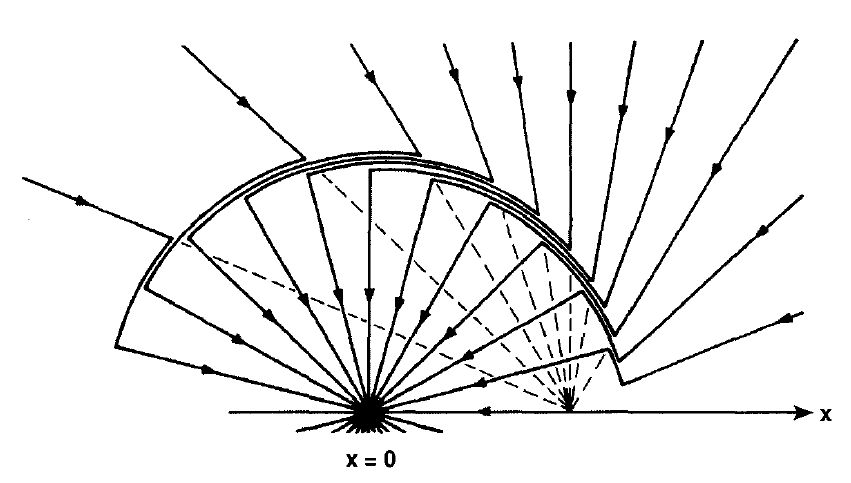
\includegraphics[width=0.8\textwidth]{\dir/figs/bremsstrahlung}
  \caption{The classical view of bremsstrahlung emission. Electric field lines are solid and dashed lines with arrows. The x-axis points to the direction of the particle movement. When the particle is abruptly stopped at x=0, two intense transverse electric fields are produced, generating an electromagnetic radiation i.e. bremsstrahlung. Adapted from \citet{haug2004elementary,asg1966berkeley}.}
  \label{bremsstrahlung}
\end{figure}

\paragraph{Laboratory micro-CT system}
A conventional X-ray source generates X-ray radiation by firing electrons onto a metal target in vacuum. The electrons were generated by thermionic emission from a heated metallic filament. The metallic filament and target are usually tungsten \citep{wildenschild2013x}. During the electrons impacting on tungsten, about 60\% of the energy is converted into heat, 39\% of the energy is lost due to backscatter, only 1\% of the input energy is converted into bremsstrahlung \citep{behling2015modern}.

There are commercial turn-key micro-CT system manufactured by a number of vendors. The turn-key micro-CT instruments have a wide range of specimen size, usually mm scale, and resolution from 100s of $\mu m$ to few $nm$. A summary of the available instruments on market can be found in the review by \citep{stock2008recent}. 

A conventional X-ray source generates cone-shaped X-ray beams, targeting a sample that mounted on a rotary stage. The X-rays are absorbed and diffracted, only part of the X-rays are able to penetrate the sample. The penetrated X-rays are captured by a detecting sensor and converted into signals (Fig.\ref{conventional}.

\begin{figure}[htbp]
  \centering
  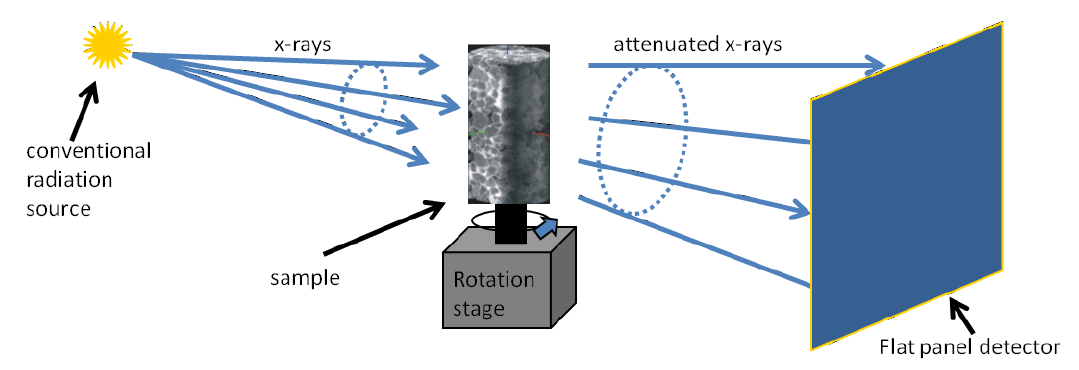
\includegraphics[width=0.8\textwidth]{\dir/figs/conventional}
  \caption{Cone beam configuration for conventional X-ray CT imaging. Cone-shaped X-ray beam is generated by an conventional X-ray source. The cone beam X-ray penetrates the sample mounted on a rotary stage and received by a detector. Adapt from \citet{wildenschild2013x}.}
  \label{conventional}
\end{figure}

\subsubsection{X-ray generated by synchrotron radiation}
Generally speaking, bremsstrahlung includes any radiation produced by decelerating a charged particle. Specifically, synchrotron radiation is a physical process of emitting radiation when charged particles being deflected in magnetic fields \citep{sokolov1966synchrotron}. Natural synchrotron radiation is called cosmic magnetobremsstrahlung \citep{ginzburg1965cosmic}. Man-made synchrotron radiation was first time observed in 1947 in the General Electric Research Laboratory in New York \citep{robinson2001history}. Synchrotron radiation can produce a wide range of  electromagnetic spectrum from infrared to X-rays. The upper limit of energy depends on the electron energy \citep{bonse1996x}. The X-ray generated by synchrotron radiation has very high emitted flux, thus the temporal resolution of synchrotron X-ray CT can be much finer than conventional X-ray CT.

\paragraph{Synchrotron light source and beam-line}
The first generation of synchrotron light sources were associated with high-energy particle colliders which primarily for particle physics studies. More recently, synchrotron light sources were built specifically for generating synchrotron radiation. 

Modern synchrotron light sources employs electron storage rings to accelerate and circulate electrons. An electron storage ring can reach a kilometre of circumference. Electrons and positrons (the counterpart of the electron) are accelerated to near the speed of light. The energy of the high-speed electrons are around 6-8 GeV, such high energy can generate extremely bright radiation that well above 10 KeV \citep{winicksynchrotron1987}. Magnetic fields are installed in the ring to steer and focus the accelerated particles. The high-speed electrons produce synchrotron radiation when they are deflected by the magnetic fields. The radiation spectrum spans widely from radio wave to visible lights, and to X-rays. The synchrotron X-ray radiation has very high photon flux and brilliance. High flux means large number of photons passing through an area in unit time, therefore imaging can be done fast, i.e. high temporal resolution. High brilliance means high intensity and directionality of the X-ray beam, therefore the X-ray beam can be focused on a small area, i.e. high spatial resolution\citep{wildenschild2013x}. Synchrotron X-ray is millions times brighter than conventional laboratory X-ray beams. The synchrotron radiation is projected tangential to the ring, and directed into each experimental station, often referred to as beam-lines (Fig.\ref{estoragering}.

beam-line consists of three major components. The synchrotron radiation exits the storage ring and enters the first component of the beam-line, the front-end. Then the radiation is filtered in the second component, the beam-line optics. The optimised synchrotron X-ray is then directed into the user's end, the experimental station \citep{wildenschild2013x}. Different beam-lines are built depending on the requirements of the study topics and imaging purposes. For example in the Advanced Photon Source in the Argonne National Laboratory (US), disciplines cover material science, biology and life science, geosciences and soil sciences, environmental science, chemistry, physics and polymer science.

\begin{figure}[htbp]
  \centering
  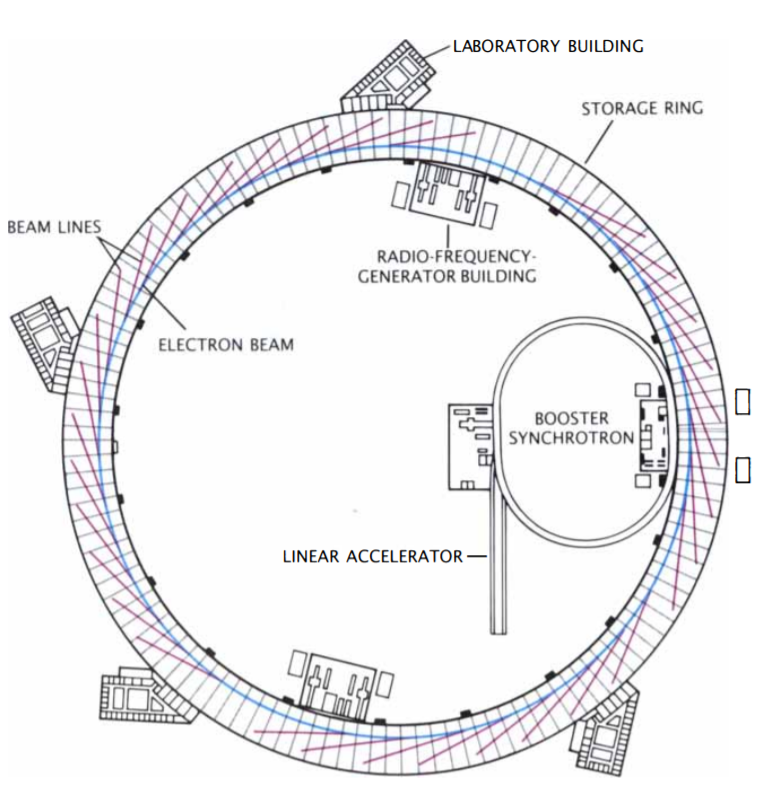
\includegraphics[width=1\textwidth]{\dir/figs/estoragering}
  \caption{A classical electron storage ring. Electrons are accelerated and stored in the ring (blue circle). Synchrotron radiation (purple lines) is produced when electrons are deflected by magnetic fields. Synchrotron radiations are guided into experimental stations that built tangential to the ring circumference. Image adapt from \citet{winicksynchrotron1987}.}
  \label{estoragering}
\end{figure}

X-ray beams generated by synchrotron radiation are parallel.  Fig.\ref{synchrotron} shows a typical synchrotron X-ray CT imaging configuration. X-ray beams pass through a monochromator, which select a narrow band of wavelengths of light, and through the target object. Penetrated X-rays are interacting with a scintillator screen that converts the X-rays to visible light, and finally reach the sensor device that converts the light into computer signals \citep{wildenschild2013x}.

\begin{figure}[htbp]
  \centering
  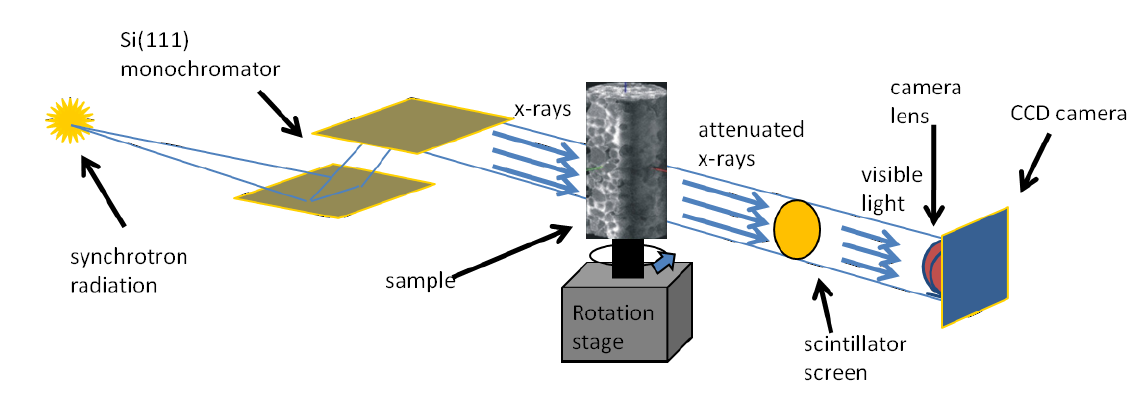
\includegraphics[width=0.8\textwidth]{\dir/figs/synchrotron}
  \caption{X-ray CT configuration of a synchrotron X-ray source. The X-ray beam from a synchrotron X-ray source is parrallel beam. The X-ray is filtered with a monochromator to obtain beam with constant energy and wavelength. The X-rays penetrates the target object on a rotary stage, and again filtered by a scintillator screen and converted to visible light. The visible light is captured by a camera. Adapt from \citet{wildenschild2013x}.}
  \label{synchrotron}
\end{figure}



\subsection{X-ray interactions with matter}
When X-ray photons interact with matter, they are absorbed, scattered, diffracted, refracted or transmitted through the material. When an X-ray photon is absorbed by an atom of the matter, electrons of the inner shell of the atom is ejected. The atom is ionised and neutralised, and emits an X-ray characteristic of the atom \citep{wildenschild2013x}. During this process of X-ray passing through the object, the X-ray intensity is attenuated. For an X-ray beam with constant energy and wavelength (i.e. monochromatic beam), this attenuation of X-ray follows the Beer-Lambert's Law:

\begin{equation}
    I=I_0exp(-\mu x)
\end{equation}

where $I_0$ is the incident X-ray intensity before passing through the object, $I$ is the attenuated X-ray intensity after passing. $x$ is the thickness of the object. $\mu$ is the linear attenuation coefficient that measures the easiness of X-ray passing through an object, higher $\mu$ means the X-ray is more attenuated after passing through an object. X-ray attenuation is majorly controlled by physical properties of the target materials and the X-ray interaction with the material. 

There are three fundamental interactions of X-ray with matter: the photoelectric effect, Compton scattering and coherent scattering (Rayleigh scattering) \citep{hsieh2003computed}. Only the first two types are important to the context of CT imaging, these two effects together decide the attenuation coefficient $\mu$:

\begin{equation}
    \mu= \tau + \sigma
\end{equation}

where $\tau$ is the photoelectric attenuation coefficient, and $\sigma$ is the Compton scattering attenuation coefficient.

\paragraph{Photoelectric effect}
The photoelectric effect was first explicated by Albert Einstein in 1905 and awarded the Nobel Prize in Physics in 1921. Fig.\ref{photoelectricandcompton} (a) illustrate a schematic process of the photoelectric effect during X-ray photon interacting with an atom. If the X-ray photon energy is greater than the binding energy of an electron of the atom, the photon contributes its entire energy to free the binding electron from an inner shell of the atom and then become vanished. The liberated electron is called a photoelectron. The inner shell is left with a vacancy for electron and thus replaced by an electron from the outer shell. This replacement of lower energy electron by higher energy electron will emit a characteristic radiation \citep{hsieh2003computed}. At low X-ray energy of 50-100 KeV, the interaction mechanism is dominated by the photoelectric effect and the attenuation coefficient $\tau$ is proportional to a power of the mean atomic number of the specimen \citep{wildenschild2013x}.

\begin{figure}[htbp]
  \centering
  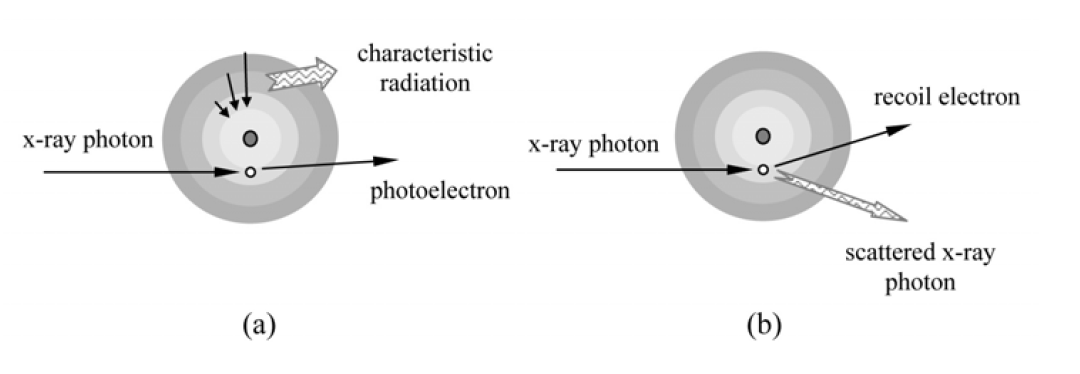
\includegraphics[width=0.8\textwidth]{\dir/figs/photoelectronandcompton}
  \caption{Photoelectric effect and Compton scattering. (a) shows the process of photoelectric effect, an X-ray photon interacts with an atom, produces a photon of characteristic radiation, a photoelectron and left a positive ion. (b) shows the process of Compton scattering, X-ray interacts with an atom, produces a scattered X-ray photon, a recoiled electron, and left a positive ion. Image adapt from \citet{hsieh2003computed}.}
  \label{photoelectricandcompton}
\end{figure}

\paragraph{Compton scattering}
Compton scattering was also a Nobel Prize-awarded (1927) finding, named after Arthur H. Compton. Fig.\ref{photoelectricandcompton} (a) illustrate a schematic process of the Compton scattering during X-ray photon interacting with an atom. This interaction is allowed to occur when the X-ray photon energy is much greater than the binding energy of an electron. The X-ray photon strikes an electron and cause it to flee from the atom. After the collision the incident X-ray photon is deflected or scattered and lost part of its initial energy. At high X-ray energy of 5-10 MeV the interaction process is via Compton scattering and the coefficient $\sigma$ is proportional to the electron density of the penetrated object \citep{wildenschild2013x, hsieh2003computed}. 

\subsection{CT image data}
\subsubsection{Grey scale images}
X-ray tomography records the intensities of X-ray attenuation of the target object, therefore X-ray μCT images are grey scale images that carry attenuation intensity information. An 8-bit grey scale image is composed of different shades of grey values ranging from black (intensity value = 0) as the weakest, to white (intensity value = 255) as the strongest intensity. In the following part of this thesis, the term intensity (if not specified else) is used to refer to grey values or brightness intensity rather than X-ray intensity. 

In the thesis, 16-bit and 8-bit images are analysed often, raw converted image from X-ray μCT are 16-bit (65536 levels) or 32-bit (4294967296 levels). Information is slightly lost during a conversion from higher bit depth to lower bit depth, but in return computational cost is reduced.

A binary image, or Boolean type data, has only two values - ones and zeros (also as Trues and Falses). Binary image is usually useful for extracting one particular feature from an image as foreground and the rest as background, for example porosity from a sandstone or pyroxenes from a gabbro. Binary images are also useful for isolating one label from multiple labels. For example isolating oil from fluids of water and oil.

\subsubsection{CT image resolution}
The spatial resolution of conventional CT is in the range of $mm$ scale. Computed X-ray micro-tomography (\textmu CT) expands CT resolution to $\mu m$-scale ($10^{-6}$ metre). The application synchrotron X-ray sources further extended the limit of spatial resolution of CT to below 1 \textmu m and enabled fast synchrotron-based X-ray \textmu CT, with scanning intervals reduced from hours to sub-seconds \citep{berg2013real}. 

High spatial resolution is crucial for higher imaging accuracy, the shape of the scanned object can be more accurately defined with higher spatial resolution, i.e. smaller pixel size (Fig.\ref{spacialres}).

\begin{figure}
    \centering
    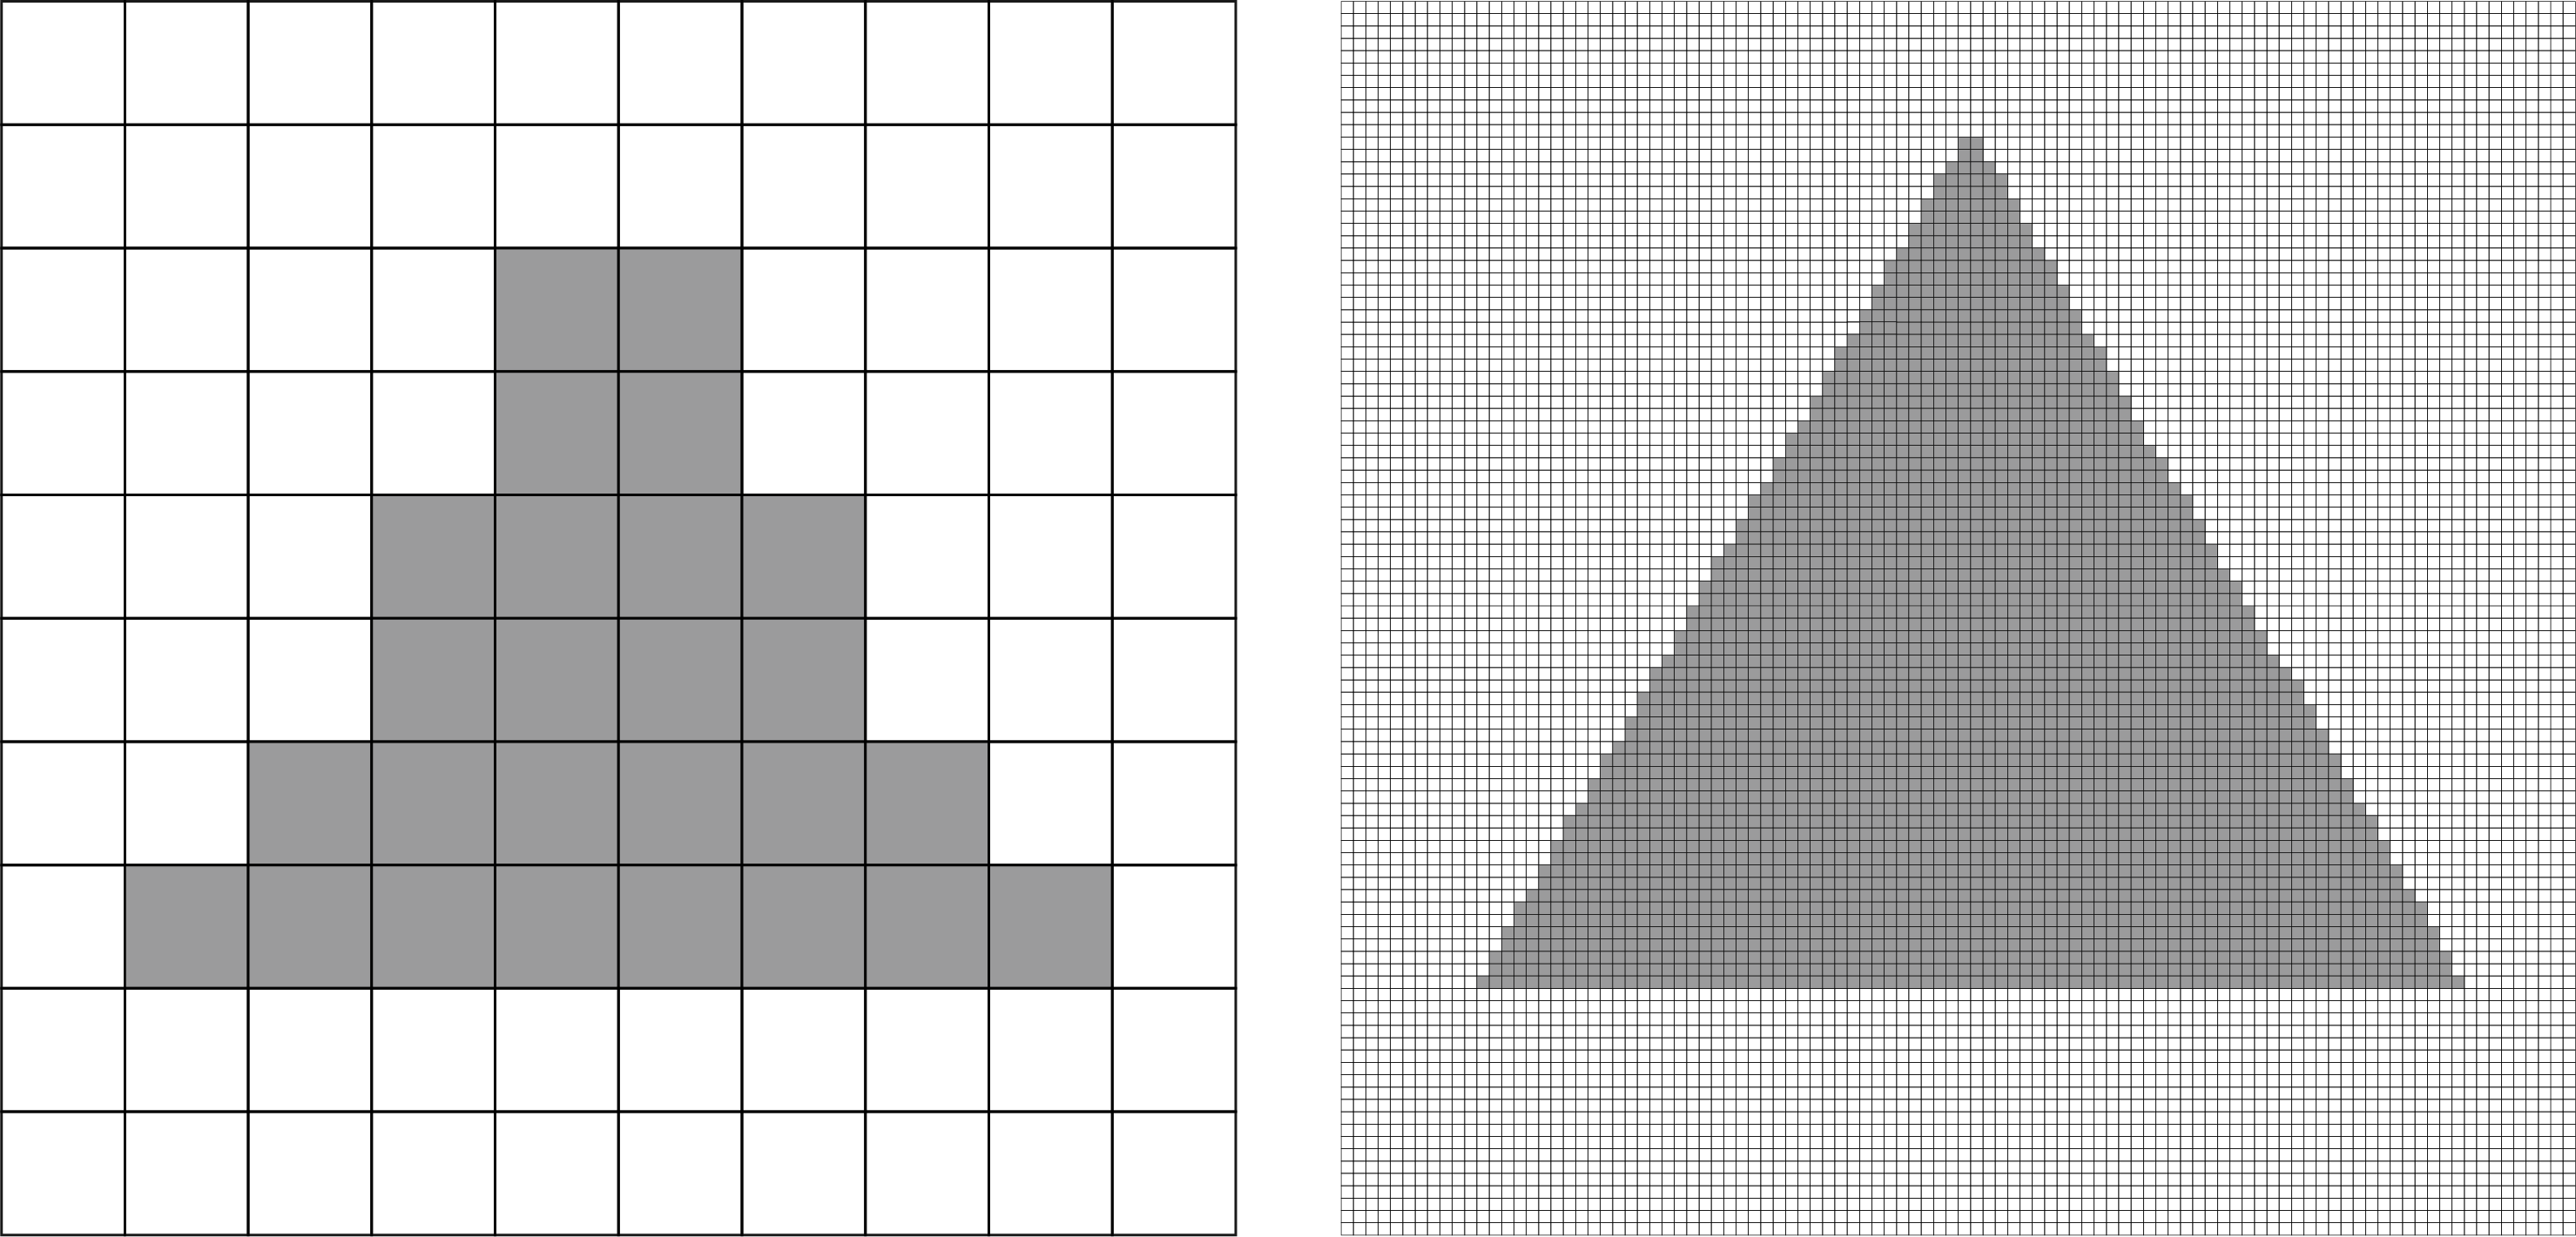
\includegraphics[width=1\textwidth]{\dir/figs/spatialresolution}
    \caption{Spatial resolution. Two triangles of same size were represented by low and high resolution. The level of proximity increase with resolution. \citep{CTscanartefacts}}
    \label{spacialres}
\end{figure}

\subsubsection{Pixel and voxel}
In digital imaging, a pixel is a value in a dot matrix data structure, and an image is a rectangular grid of pixels (Fig.
\ref{pnv} left figure). Pixels are square, and are the smallest element of a digital image. The length of pixels of a picture is defined by its resolution, higher resolution leads to smaller pixels. In X-ray μCT imaging, a pixel records the attenuation intensity of a finite point of the target object, and the intensity is represented by a grey scale value.
 
A voxel is a three-dimensional equivalent of pixel (Fig.\ref{pnv} right figure). Voxels represent values in three-dimensional space, and the position of a voxel is located by a three-dimensional Cartesian coordinate system. 

\begin{figure}
    \centering
    \includegraphics[width=1\textwidth]{\dir/figs/pixelnvoxel}
    \caption{Pixel and voxel. Left figure: pixels with different values in a 2D Cartesian coordinate. Right figure: voxels with different values in a 3D Cartesian coordinate \citep{CTscanartefacts}.}
    \label{pnv}
\end{figure}

\section{CT image processing part I: reconstruction and denoise}
\subsection{Overall workflow}
Image processing aims at identifying the objects presented in the image. A general CT image processing work flow is summarised in Fig.\ref{ctworkfl}. This work flow is abstracted from this study, the work flow may vary from different CT data sets as different imaging condition are applied and different demands for analysis required. In the following section the generic introduction of the CT image processing workflow is explained. The details of the specific work flow used in this study is further explained in the methodology chapter. In this chapter, the overall CT image processing workflow is introduced in two parts, the first part will start from image processing of data that directly acquired from CT instrument - projection images, to a more straight-forward representation of the imaged object - reconstruction images (the first row of blocks in Fig.\ref{ctworkfl}) . The second part will focus on extracting pragmatic information from the reconstruction images by segmentation, visualisation and measurements (the second row of blocks in Fig.\ref{ctworkfl}).

 \begin{figure}[htbp]
  \centering
  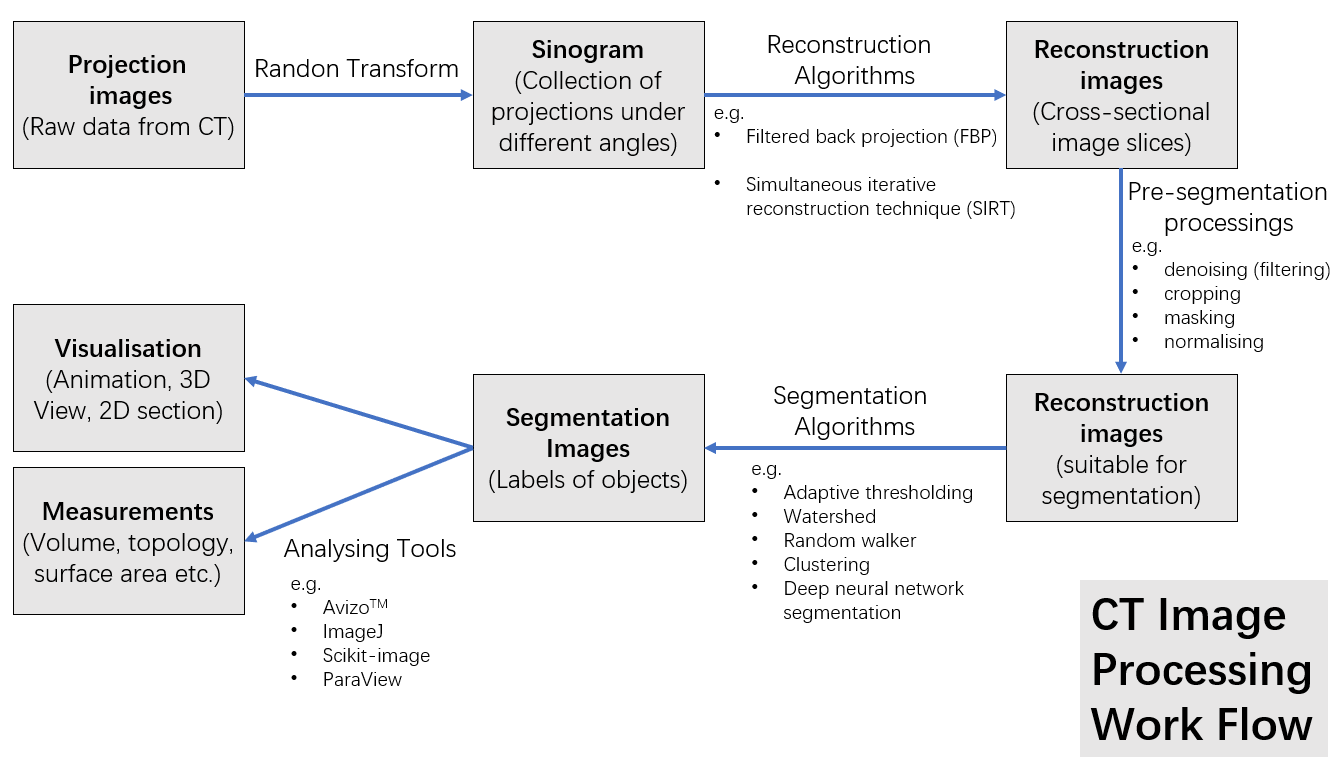
\includegraphics[width=1\textwidth]{\dir/figs/ctworkfl}
  \caption{A general summation of CT processing workflow used in this study. The projection images were converted into sinograms and Reconstructed images. The reconstructed images are segmented into labelled images that represent oil, brine and rock of the scanned object. Visualisation and measurements can then be carried out on the labelled segmentation images.}
  \label{ctworkfl}
\end{figure}

\subsection{Projection images} 
Raw data acquired from X-ray tomography are called projections images (or simply projections), they are X-ray projections of the target object from one particular angle. During an X-ray CT imaging process, the target object is imaged over a rotation of 360 degrees (for cone-beam instruments, but only 180 degrees for a parallel beam synchrotron set up), with step angle $\omega$ (Fig.\ref{ctrotangle}). The intensity of the penetrating X-rays are captured by a sensor device, and then processed into digital signals. These raw data acquired from X-ray tomography are called projections images, they are X-ray projections of the target object from one particular angle. The Projection images essentially carry information about the difference of X-ray absorption inside the object. Fig.\ref{psr} (A) shows one projection image (X-Y plane) from a micro CT scan of a cylinder carbonate rock sample.

\begin{figure}[htbp]
  \centering
  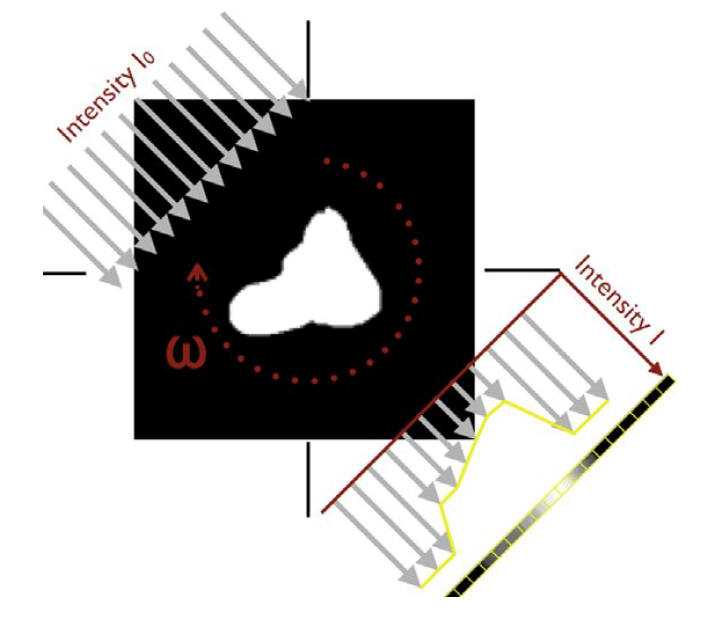
\includegraphics[width=0.8\textwidth]{\dir/figs/ctrotangle}
  \caption{Acquisition of CT projection. X-ray beam with initial intensity $I_0$ is attenuated by the object, the penetrating X-ray intensity $I$ is recorded as a line of pixels. This process is repeatedly carried out from $0-2\pi$ with rotation step$\omega$. Adapted from \citet{fusseis2014low}.}
  \label{ctrotangle}
\end{figure}

\subsection{Sinogram}
The collection of projections from different angles around the objects can be represented by sinograms that shows the absorption intensity signal at different rotation angles. This process is essentially the mathematical operation of Radon transform \citep{radon20051} of the projection image. 

\begin{figure}[htbp]
  \centering
  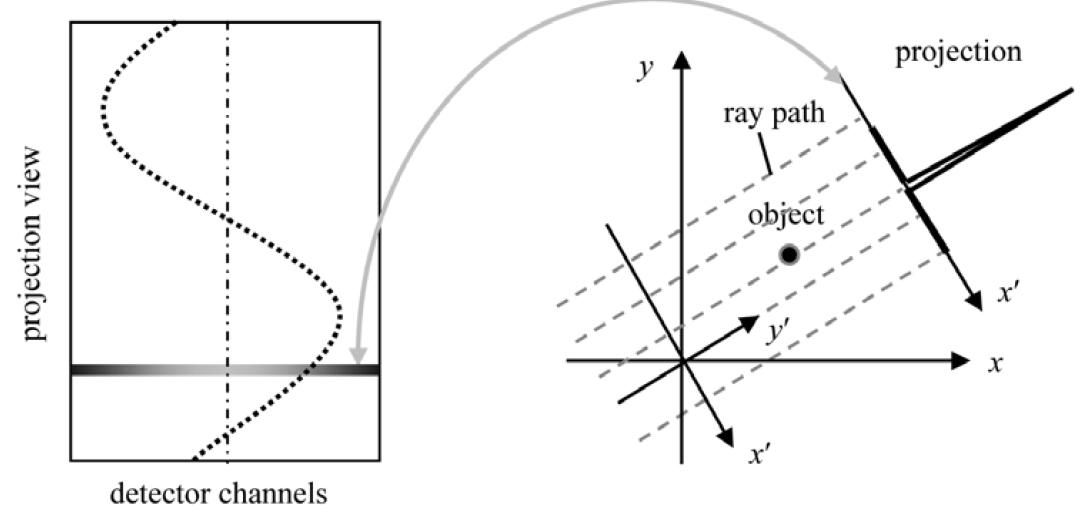
\includegraphics[width=0.8\textwidth]{\dir/figs/sinogram}
  \caption{Schematic diagram of the mapping between the sinogram space and the object space. A fixed point on the scanned object is represented as a sinusoidal curve. A single projection from a particular angle is represented as a horizontal line on the sinogram. Image adapted from \citep{hsieh2003computed}.}
  \label{sinogram}
\end{figure}

Fig.\ref{sinogram} shows schematic diagram of the mapping between the sinogram space and the object space. In the sinogram space, the X-axis represents the detection channels and the Y-axis represents the projection angle. There are two ways to interpret a sinogram. First, for a fixed point on the target object (shown as black dot on the right figure), its value of projection from different angles is recorded on the sinogram that forms a sinusoidal curve (left figure dotted curve). Another perspective to look into a sinogram is a line parallel with the X-axis, this line represent the intensity record of a single projection. Fig.\ref{psr} (B) shows the sinogram converted from the projection images. 

\begin{figure}[htbp]
  \centering
  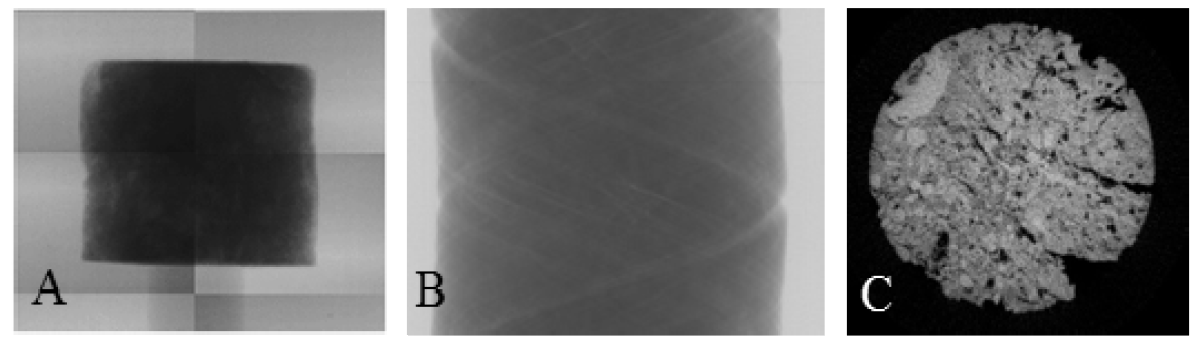
\includegraphics[width=0.8\textwidth]{\dir/figs/psr}
  \caption{Example of projection (A), sinogram (B) and reconstruction image (C) taken from a CT scan of a carbonate rock. \citep{Pak2014thesis}}
  \label{psr}
\end{figure}

\subsection{CT reconstruction}
Projections are a collection of X-ray measurements, of which each presents a summation of the attenuation coefficient of the object along a particular path of the X-ray beam. CT reconstruction is mathematically a inverse problem, of which the objective is to estimate the attenuation distribution of the imaged object using these measurements. By reconstruction, the projections are reconstructed into two-dimensional image slices (horizontal cross-sections) of the object (Fig.\ref{psr} (C)). CT image reconstruction is complicated due to various of factors and trade-offs such as the trade-off between spatial resolution and sample size, temporal resolution and noise, computational complexity and artefacts etc. Here only a brief overview of CT reconstruction relevant to this study is provided.

\subsubsection{Fourier transform and Fourier slice theorem}

Before introducing any reconstruction algorithm, first of all I will briefly introduce the Fourier transform, and the theory that governs tomographic reconstruction - the Fourier slice theorem \citep{kak2001principles} - in an intuitive explanation. 

Fourier transform is essentially a mathematical transform that decompose a signal function into constituent frequencies. It can present every non-linear function (e.g. an image, a song can all be seen as non-linear functions) by a sum of sine and cosine waves. For example, a photograph of a dog that human can recognise is in its spatial domain, where each pixel forms the shape of a dog. The photograph can be equivalently represented in the frequency domain that each point represents a particular frequency of the spacial domain image by performing Fourier transform.

The Fourier slice theorem states that: 

\begin{quote}
The Fourier transform of a parallel projection of an object $f(x, y)$ obtained at angle $\theta$ equals a line in a 2D Fourier transform off $f(x, y)$ taken at the same angle.
\end{quote}

In plain words, it implicates that, by performing 1D Fourier transform on each projection, we obtain a line in the 2D Fourier transform of the object. To fill the entire Fourier space of the object being reconstructed, we need a sufficient number of projections that surround the object from angle $0-\pi$. The complete Fourier space information can be used to recover the object by performing inverse Fourier transform.

\subsubsection{Filtered back-projection method}
The widely used reconstruction method is the filtered back-projection (FBP, \citet{herman1976convolution}), it has the balance of quality and efficiency therefore became the conventional method for reconstruction. The filtered back-projection method is based on the Fourier slice theorem (Fig.\ref{fbp}). In order to reconstruct the object using the theorem, we need to perform inverse Fourier transform on 2D Fourier transform of the object. The 2D Fourier transform is obtained by 'patching together' all 1D Fourier tranforms. For a cylindrical object, ideally we want the 1D Fourier transform of circular sector shape (Fig.\ref{fbp} (a)), because that would prevent any overlapping when 'patching together' all 1D Fourier transforms. Realistically, the 1D Fourier transform is rectangle shaped (Fig.\ref{fbp} (b)). Simply summing up the 1D Fourier transforms will cause overestimation in the centre of the cylinder but underestimation on the peripheral of the cylinder. To solve this problem, the rectangle shaped 1D Fourier transform is multiplied by a weighting function ((Fig.\ref{fbp} (c)) to approximate the ideal shape (a).

\begin{figure}[htbp]
  \centering
  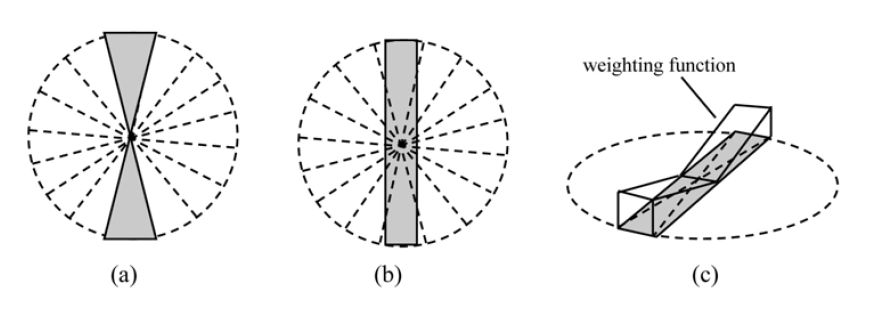
\includegraphics[width=0.8\textwidth]{\dir/figs/fbp}
  \caption{Conceptualised illustration of filtered back-projection method. (a) is idealised shape of area to use 1D Fourier transform. (b) is realistic shape of area to use 1D Fourier transform. (c) is realistic area optimised with a weighting function to approximate the ideal shape (a). Image adapted from \citet{hsieh2003computed}.}
  \label{fbp}
\end{figure}

\subsection{Artefacts in reconstructed CT images}
Artefacts are systematic discrepancies between the reconstructed image and the true image \citep{barrett2004artifacts}. In CT derived images, artefacts are essentially discrepancies between the reconstructed values in an image and the genuine attenuation coefficient of the object. Artefacts can occur as streaking, shading, rings and distortions etc., and to some extent degrade the quality of CT images. Artefacts are produced both at the CT data acquisition stage, by intrinsic physical processes and imperfections in the CT instrument, and at the data reconstruction stage. Artefacts can be avoided, corrected or alleviated by proper methods. All artefacts affect the absolute grey scale distribution of an image, and so must be avoided if good image classification is to be achieved.

\subsubsection{Physics-based artefacts}
Physics-based artefacts are generated from physical processes of CT scanning, such as the absorption of the X-ray beam. 

\paragraph{Beam Hardening}
The mean energy of a poly-chromatic X-ray beam increases (becomes "harder") as the beam penetrates an object due to faster absorption of the lower-energy photons; this is beam hardening. Beam hardening mainly produces cupping artefacts for cylindrical samples, where the  total brightness of the X-ray beam is reduced by adsorption of low energy photons in the middle of the cylinder than it in the peripheral of the cylinder. This leads to a characteristic cupped-shaped X-ray intensity profile along the cylinder. In very heterogeneous samples, beam hardening can also lead to streaks and dark bands. Beam hardening can be minimised by using filtration, calibration correction and beam hardening correction software, or avoided by using monochromatic beams at Synchrotron facilities \citep{barrett2004artifacts}.

\begin{figure}[htbp]
  \centering
  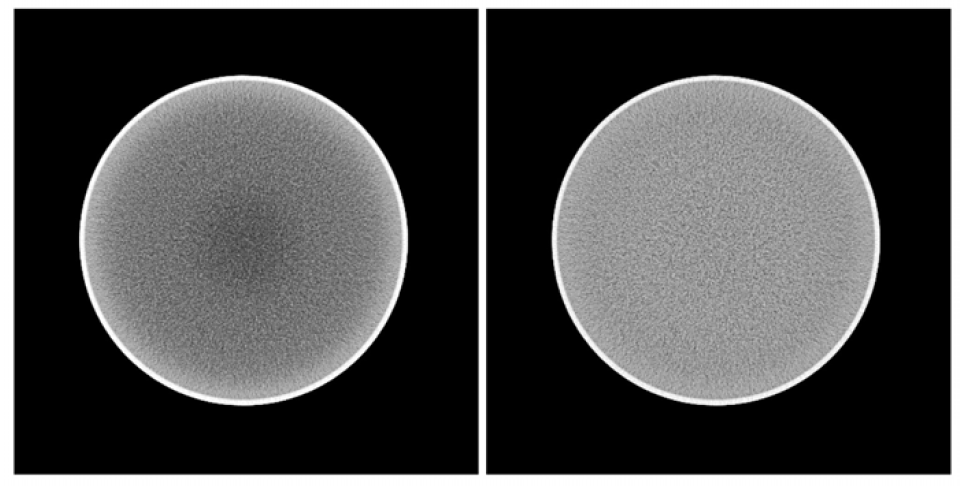
\includegraphics[width=0.8\textwidth]{\dir/figs/bh}
  \caption{ Reconstructed images of a 35-cm water phantom. Left figure shows cupping artefact caused by beam hardening. Right figure shows CT reconstruction image without beam hardening. Image adapted from \citep{hsieh2003computed}.}
  \label{bh}
\end{figure}

\paragraph{Partial Volume effect}
Partial volume effect (Fig.\ref{pve}) refers to the phenomenon that the grey scale value of a pixel/voxel is a representative of the average attenuation of the materials within a voxel \citep{barrett2004artifacts}. It is due to that inside the size of one voxel there exists more than one material with different attenuation coefficients. The effect can cause the appearance of artefacts such as shading and blurring. Increasing the spatial resolution of CT can alleviate this problem, i.e. containing more than one material within a voxel occurs less frequently when the size of the voxel is smaller. This effect can not be eliminated.

\begin{figure}
    \centering
    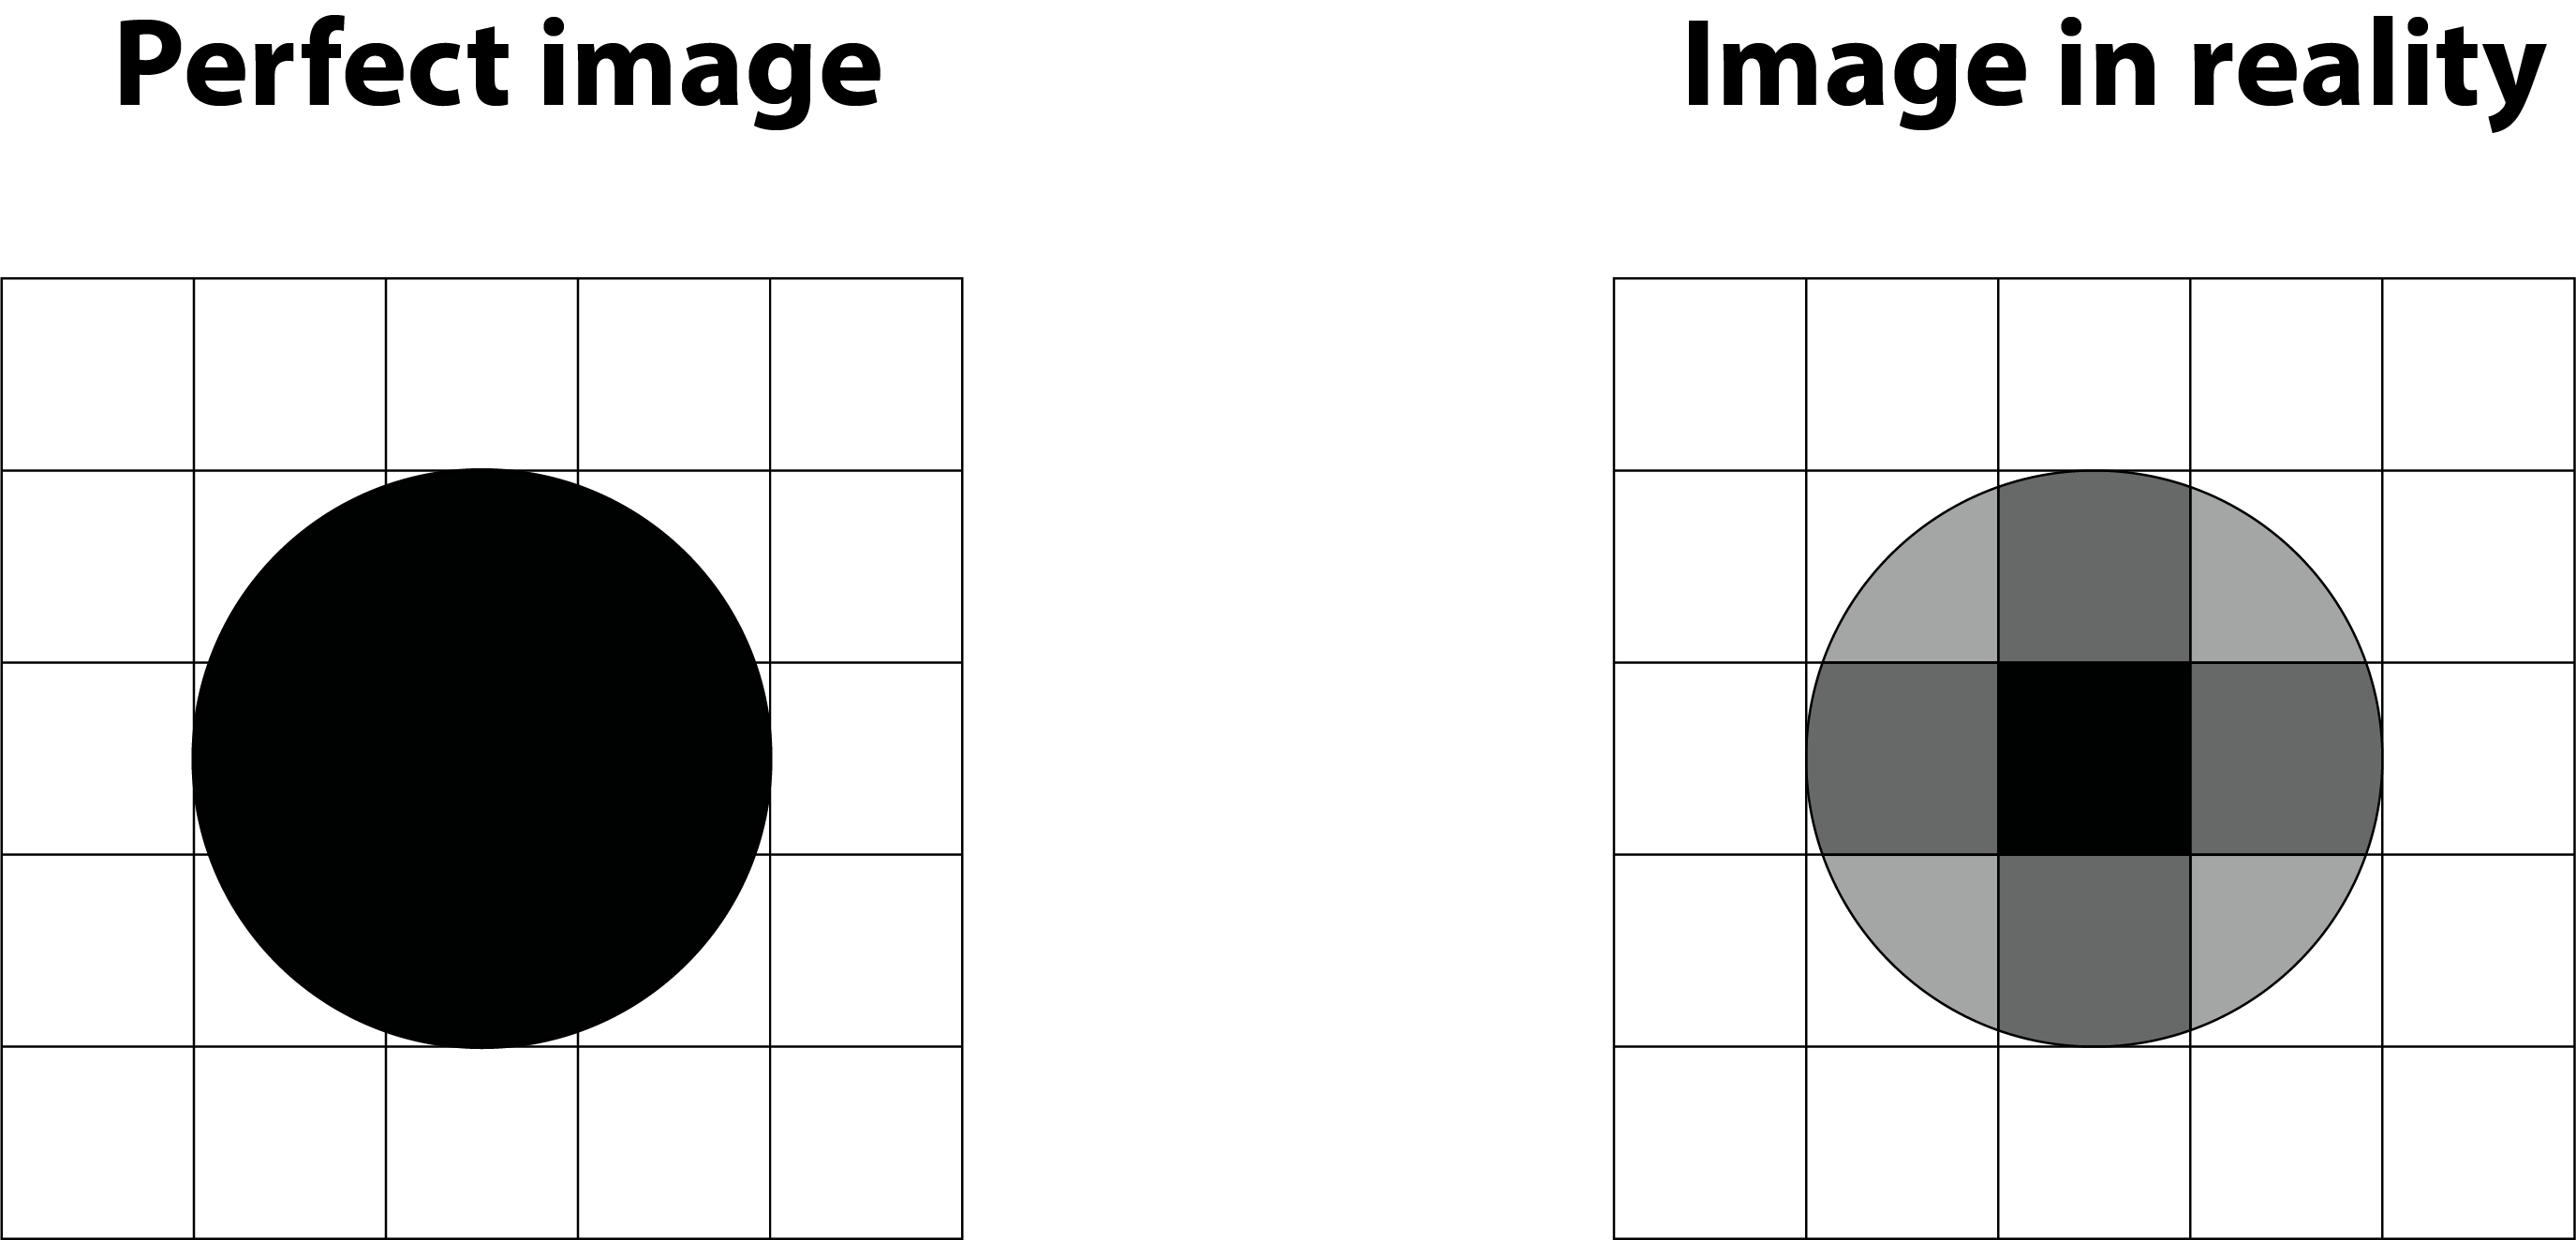
\includegraphics[width=1\textwidth]{\dir/figs/partialvolume}
    \caption{Partial volume effect of a solid circle. Left figure shows the perfect image without partial volume effect. Right figure shows realistic image that the pixels on the border of the circle containing two phases, therefore their intensity are averaged by the circle and the outside. Image adapted from \citep{CTscanartefacts}.}
    \label{pve}
\end{figure}

\paragraph{Under-sampling} 
Under-sampling happens when the angular intervals between projections are too large. It produces aliasing that appears as fine radiating stripes. Aliasing can be minimised by acquiring a larger number of projections per rotation \citep{barrett2004artifacts}. The fine, radiating stripes that at a distance from the object is called view aliasing, and the stripes that close to the object is called ray aliasing (Fig.\ref{undersamp}).

\begin{figure}
    \centering
    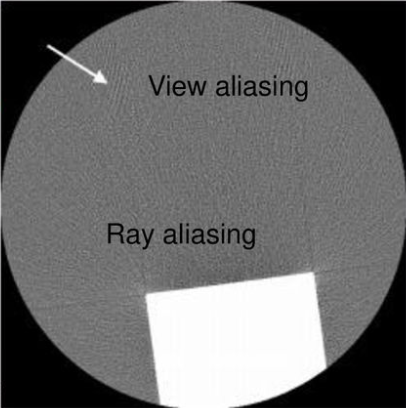
\includegraphics[width=0.6\textwidth]{\dir/figs/undersamp}
    \caption{View aliasing and ray aliasing of a cube phantom caused by undersampling. View aliasing occurs a distance away from the object. Ray aliasing occurs close to the object. Image adapted from \citep{CTartifacts}.}
    \label{undersamp}
\end{figure}

\paragraph{Photon Starvation} 
When the X-ray beam attenuation is too high, or the X-ray beam is too sparse thus photons recorded by the camera are insufficient, highly noisy projections are produced. This is called photon starvation. It usually leads to streaking artefacts \citep{barrett2004artifacts} (Fig.\ref{photonstarvation}). In most of the geo-scientific studies, photon starvation can be overcome by increasing the X-ray energy, as it is unnecessary to consider X-ray dose.

\begin{figure}
    \centering
    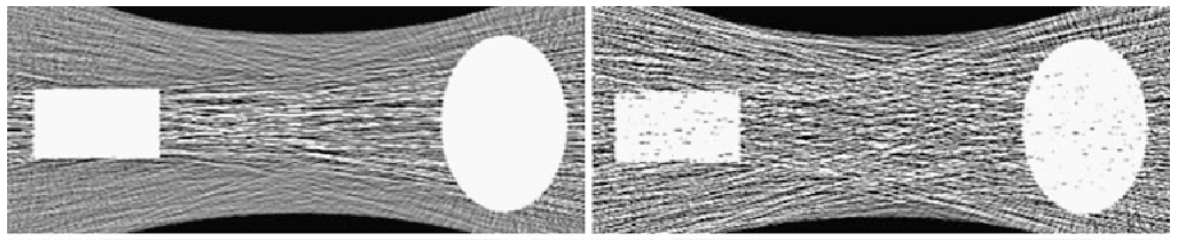
\includegraphics[width=1\textwidth]{\dir/figs/photonstarvation}
    \caption{Photon starvation artefact in a CT image of a rectangle phantom and a ellipsoid phantom. Left figure and right figure are scanned with X-ray beam of 225,000 and 40,000 photons per ray. The right CT image with less photons per ray appears more noisy. Image adapted from \citep{mori2013photon}.}
    \label{photonstarvation}
\end{figure}


\subsubsection{Hardware-based artefacts}
\paragraph{Ring artefacts} 
Ring artefacts are concentric circle artefacts. They are very common in CT scans and mostly due to non-linear behaviour of individual camera pixels, i.e. the output response to input from the camera scintillator is out of step with the neighbouring pixels. Radiation damage also can lead to bad pixels. Ring artefacts can be minimised by re-calibration, or using filter software.

\begin{figure}[htbp]
  \centering
  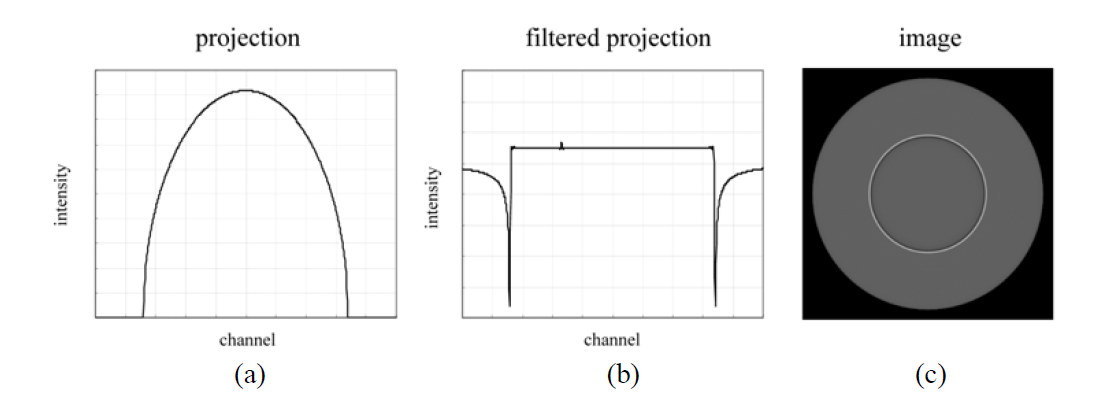
\includegraphics[width=1\textwidth]{\dir/figs/ring}
  \caption{Artificial ring artefact. About 1\% of error was added to a single channel over all projection angles. (a) Projection profile with 1\% added error. (b) Profile after filtering operation. (c) Reconstructed image with a bright ring artefact in the middle. Image adapted from \citet{hsieh2003computed}.}
  \label{fbp}
\end{figure}

\subsection{Noise in reconstructed CT images and denoising methods}
Noise is a random, variation of grey values in images. Unlike artefacts, noise does not inherent to the CT imaging process or the CT instrument, but inherent to the more generalised process of electric signal processing. Noise is produced in multiple ways, the generation of noise and denoising methods are extensively studied in data science and signal processing science.

\subsubsection{Source of noises}
There are four major sources of noise: random noise, statistical noise, electronic noise and round off mistakes \citep{diwakar2018review}.

\paragraph{Random noise} 
Random noise is generated by activities in the environment where X-ray CT scan is being carried out. Random noise is also referred to as 'white noise', because like the colour white that includes all the colours of a spectrum, white noise contains all frequency harmonics in approximately equal magnitude. 

\paragraph{Statistical noise}
During the transmitting of a finite number of X-ray photons, the number of photons detected by the camera device may vary between measurements because of statistical fluctuation. For pixels that receive photons via beam paths that have the same total attenuation, the number of photons recorded is not identical but is represented by a population. This is known as statistical noise, or quantum noise. That population gets narrower as the total number of photons detected increases. Statistical noise is reduced by increasing the number of detected photons.

\paragraph{Electronic noise}
The electronic circuits that detecting the analogue signal have inherent noise, like electromagnetic interference, thermal agitation or radio frequency interference. These noise can affect the process of receiving X-ray signals. This is the electronic noise. It is minimised by carefully engineered CT instrument.

\paragraph{Round-off errors}
All X-ray signals are ultimately processed by computer. So there is inevitable process of converting signals from binary system to decimal system. Due
to limited number of bits for storage of discrete signals in computer system, the mathematical computations have to involve round-off operations. The noise brought by round-off operations is round-off error\citep.

Reconstructed CT images may be affected by a mixture of noises from the above sources. But in general, the noise distribution in CT images can be characterised by Poisson distribution or Gaussian distribution \citep{diwakar2018review}.

\subsubsection{Denoising methods}
CT derived images generally have some degree of noise. It is assumed that an image with noise is the summation of the desired image and a noise component \citep{diwakar2018review}. Noise affects the quality of the CT image therefore can cause problems during analysis of the image data. Denoising is the task of reducing the noise component as much as possible, while preserving the original image pattern to recover the desired image. In this section some frequently used denoising methods are introduced, for further knowledge \citet{diwakar2018review} provid an extensive and detailed review on denoising methods.

\paragraph{Median Filter} Random noise in CT images can be reduced by using denoising algorithms as known as filters. The most common type of filters are local smoothing filters (also known as neighbourhood filters). This kind of filters restores a pixel by taking average of its neighbouring values. Taking a $3\times3$ median filter \citep{huang1979fast} as example (Fig.\ref{median}), a window size of $3\times3$ pixel is sliding across the image, and the value of the central pixel is replaced by the median of the greyscale values of the 9 values. One benefit of using the median rather than mean (known as mean filter) is that outlier values can significantly affect the mean value but not the median value. This algorithm can significantly reduce the outlier noise and therefore 'smooth' the noisy image. Though simple and fast, the median filter smooths the entire image regardless of the boundary pattern of objects. 

\begin{figure}[htbp]
  \centering
  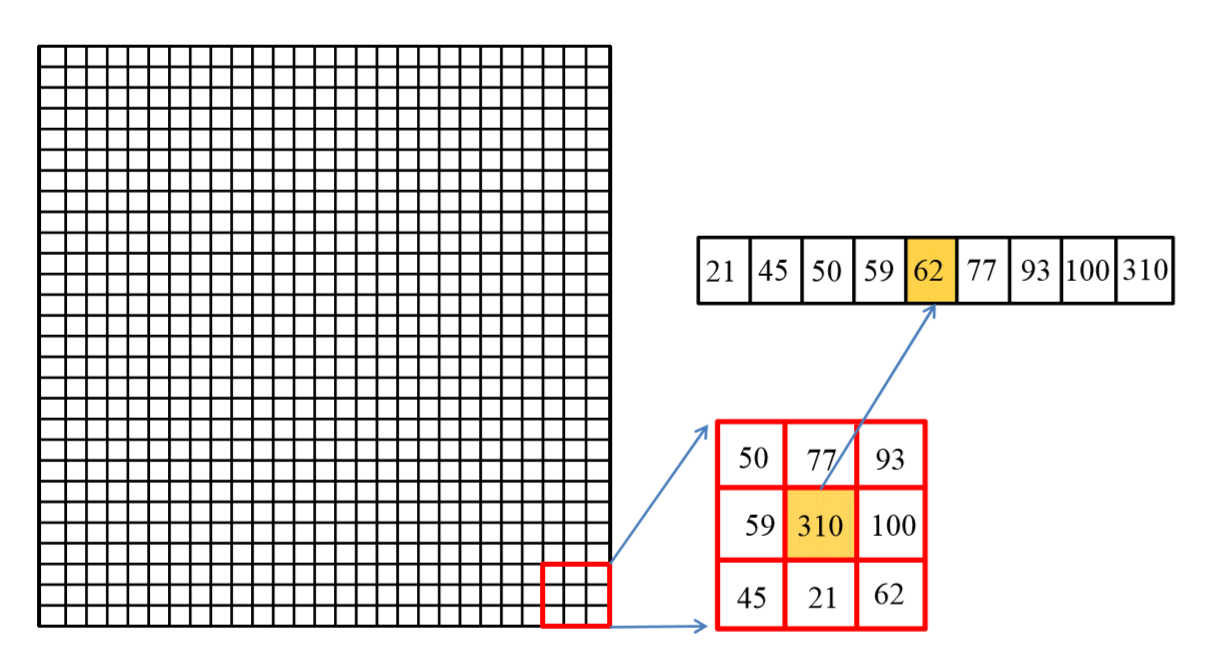
\includegraphics[width=1\textwidth]{\dir/figs/median_filter.png}
  \caption{Application of a 3x3 median filter on a 2D image. The red matrix shows the kernel and its neighbourhood window. The median number 62 was taken as the filtered value of the kernel. Image from \citet{Pak2014thesis}.}
  \label{median}
\end{figure}

\paragraph{Bilateral filter}
Median and mean filters have the major problem of obscuring the boundaries and small features of image patterns. \citet{tomasi1998bilateral} introduced the bilateral filter which removes noise while preserving the boundaries. The bilateral filter takes the geometric closeness and photometric similarity of the pixels inside/outside the window into account, and replaces the pixel value with an average of similar and nearby values.

The bilateral filter defines similarity functions that measures both the geometric closeness and photometric similarity. In 'smooth' regions i.e. inside a image pattern that does not include boundaries, the bilateral filter acts the same as the mean filter. When a sharp boundary presents in the window, the similarity functions splits the window into two sides defined by the boundary. As a consequence, the smoothing only affects either side and the boundary is preserved.

However, \citet{buades2011non} questioned the approach with the idea that '\textit{the most similar pixels to a given pixel have no reason to be close at all}'. He introduced a similar but more advanced and increasingly used filter called the 'non-local means' filter \citep{buades2011non}. The non-local means filter is adopted in this study and is introduced in chapter three.

\paragraph{Other methods}
In this study various of denoising filters were tested on the data, in this section I will briefly introduce the methods that have been tested. The methods introduced above belong to the category of spatial domain filtering, i.e. by applying filters directly on original noisy image. In this category, there are other denoising algorithms which practise the least square fidelity minimisation concept \citep{yan2011new, yan2011power,yan2012smoothed}. To name a few Tikohonov \citep{tikhonov1978methods}, anisotropic diffusion \citep{perona1990scale}, total variation \citep{chambolle2004algorithm} methods and the combined anisotropic total variation \citep{rudin1992nonlinear} method. Another category parallel with the spatial domain filtering is the transform domain filtering. Rather than directly filter the original noisy image, the noisy image is decomposed into different frequency components called wavelets (i.e. wavelet transform \citep{mallat1989theory}). The widely studied domain in this category is the non-linear coefficient thresholding based methods \citep{mallat1989theory}. With the state-of-art deep learning algorithms being powerful in solving image-related problems, convotional neural network (CNN) denoising approaches are increasingly investigated (e.g.\citep{kang2017deep,chen2017low,chen2017low2,gondara2016medical}).


\section{CT image processing part II: Segmentation}
To analyse and quantify X-ray μCT derived geological images, different constituents, for example intensities or textures, on the image needs to be classified into non-overlapping regions that represent oil water and solid. This process is called segmentation, it is the major processes in analysing and extracting quantitative information relating to the properties of the digital images. The quality of segmentation critically affects the downstream analysis of the scientific process.

However, there are some factors that influence the quality of the images, thus cause difficulties in segmentation. First, natural geological samples are usually highly heterogeneous in both mineralogy and geometry, this leads to usually sub-resolution features that cannot be identified. Second, CT images are affected by partial volume averaging, where the greyscale value of a voxel is the average of the values within a voxel, thus distorts the image \citep{barrett2004artifacts}. Third, instruments caused artefacts and noises. These problems can be wholly or partially alleviated by a pre-processing step before segmentation. Additionally, the data produced by X-ray μCT are essentially recordings of attenuation values that are uncalibrated with respect to actual composition, and the information is interpreted by human observation with other supporting observations such as Electron Microprobe Analysis (EMPA) and Scanning Electron Microscope (SEM). This means that discrepancy in different interpretations will also affect the segmentation. 

In practice, one or a combination of segmentation algorithms is used to assign every pixel with a label, so pixels with the same label are in the same category. Categories are usually defined according to the interpretation of the image, such as different mineral phases or different parts of a fossil. The outcome of image segmentation is a map of labelled areas that shows the spatial distribution of different objects. 

\subsubsection{Segmentation methods}
By Khan’s (2013) classification, image segmentation methods can be classified into six major categories. They are: 1) Threshold based; 2) Region Based; 3) Edge based 4) Fuzzy Theory based 5) Artificial Neural Network (ANN) based and 6) Partial Differential Equations (PDE) based. A segmentation algorithm is a set of computer operations that execute the segmentation methods. This section introduces major segmentation algorithms tested and related with the work described in this. 

\paragraph{Thresholding}
CT images consist of pixels that record the X-ray attenuation which reflecting the density and mean atomic number of the object and the energy of the incident X-rays. Therefore the main difference between different materials is the intensity value of the pixel. Thresholding is the most straight-forward, intensity-based segmentation method. By choosing an intensity threshold, the intensity values above and below the threshold are separated into two domains. Either domain represents one of the materials to be segmented. 

For the ideal case, where the intensity values of two different materials do not overlap at all, thresholding is easy and straight-forward. However for most real cases, two intensity distributions almost always overlap to some extent due to artefacts, noises and potentially compositional variations. Therefore, segmentation by thresholding often mis-classify the overlapped intensity (Fig.\ref{thresholding}). Nonetheless, for CT images with good contrast and low noise, thresholding is generally a good choice.

\begin{figure}[htbp]
  \centering
  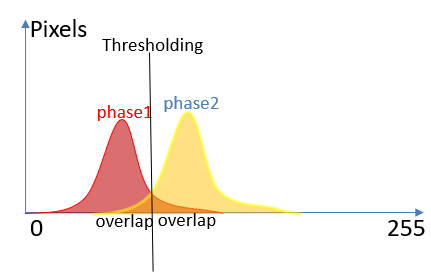
\includegraphics[width=1\textwidth]{\dir/figs/thresholding.png}
  \caption{Schematic illustration of thresholding an 8-bit image. Two phases on the image have different but partly overlapped distribution of intensity (red and yellow). By defining a threshold value the two phases are roughly separated, however thresholding can not handle the overlapping part of the intensity distribution. Therefore these pixels with overlapping intensity are mis-classified.}
  \label{thresholding}
\end{figure}

The optimal thresholding value can be chosen by trail and error. There are also automated algorithms for thresholding, the mostly used ones are Otsu method \citep{otsu1979threshold} for 2-phase thresholding and K-means clustering \citep{ridler1978picture} for multi-phase thresholding. 

In some CT images, the same material can have varied contrast due to intensity fluctuation by artefacts and noises. The variation can occur across different CT batches, or across different image slices, and even different regions within a single image. In this case there exists no single 'global' thresholding value that can be applied to all regions/images. This problem can be solved by adaptive thresholding (e.g. \citet{sauvola2000adaptive},\citet{niblack1986introduction})that uses local information to calculate the thresholding values for different regions. 

In conclusion, thresholding is the simplest of the common segmentation methods, however it has the shortcoming of low tolerance to noise and artefacts. The direct use of thresholding on CT images often leads to vast mis-classification. For CT images with less ideal quality, more advanced segmentation methods are proposed.

\paragraph{Watershed}
Watershed is one of the mostly used segmentation algorithms in CT image processing. It is a region-based segmentation method originated on the theory of mathematical morphology \citep{serra1986introduction}.

In a CT image, there are pixels with high and low intensity values distributed as patterns. In watershed segmentation, the image is regarded as a topographic landscape, where the maxima of intensity values represent "ridges" and the minima of low values are "valleys". The elevations of this landscape are defined by grey values or the gradient magnitudes of individual pixels. With this idea, the image is decomposed into numbers of non-overlapping \textit{catchment basins} separated by \textit{watersheds}. Then the \textit{catchment basins} are mathematically "flooded" such that some regions on the image begin to merge. The merging is supported by a method called \textit{merge tree} to characterise the best level of merging. The image is segmented when the best level of merging is achieved.

Marker-based watershed method allows users to explicitly define specific positions, usually local maxima/minima, to produce better segmentation. 

\paragraph{Random walker}
Random walk is a mathematical problem raised by K. Pearson in 1905. The random walker is a segmentation algorithm based on solving the Dirichlet problem, adapted to image segmentation by \citet{grady2006random}. It uses pre-labelled pixels as markers, and judges segmentation by the highest probability that unlabelled pixels reach pre-labelled pixels by random walks. The random walker is formulated in discrete space thus allowing it to be performed in arbitrary dimensions. This algorithm is extensively used in this study and will be introduced in detail in the methodology chapter (Chapter three).

\paragraph{Deep learning segmentation}
The state-of-art deep learning algorithms, especially the convolutional neural network (CNN), have been proved effective in image-related tasks in a revolutionary way. It is essentially a segmentation method by training a model classifier using a vast number of labelled data. In this thesis I implemented the convolutional neural network on CT image segmentation and increased the segmentation efficiency from hours to minutes for a single CT volume comparing with conventional segmentation routine. The detail of this method is described in Chapter four.

\subsection{Measurements of CT derived geological images}
The segmented CT images are ready for quantification and scientific analysis. There are numbers of measurements that are useful in geological CT image analysis.

\paragraph{Representative elementary volume}
Representative Elementary Volume (REV) is the smallest unit volume over which measurements can represent the whole sample. Sample REV has to be at least no larger than the targeted volume to show a representative result. 

\paragraph{Volume}
The volume of the void space in segmented images can be directly measured as the porosity, the measurement is always smaller than the genuine porosity due to the exclusion of sub-resolution micro-porosity that can not be clearly imaged. Volume of fluids can be directly measured, and therefore the fluid saturation can be derived as the ratio of fluid volume to porosity.

\paragraph{Pore network characteristics}
Pore network characteristics can be directly measured from the segmented images, or indirectly measured by pore network modelling methods. The characteristics includes porosity, absolute and relative permeability, pore aspect ratio (the ratio of longer axis to shorter axis of a pore), pore size distribution, surface area and connectivity of the pore network.

\paragraph{Curvature}
Curvature measurement is important for fluid flow in porous medium, as it is the important property from which can be derived the capillary pressure. Curvature for a point on a 2D curve is simply the inverse of its inscribed radius. Curvature for a point on a 3D surface has two independent principal curvatures. Curvatures are difficult to measure and are extremely sensitive to noise and artefacts \citep{wildenschild2013x}. \citet{armstrong2012linking} measured oil-water interfacial curvature in drainage-imbibition cycles. They estimated capillary pressure via the Young-Laplace equation and the estimation shows good agreement with experimental measurements from a pressure transducer. \citep{andrew2015imaging} measured $CO_2$-brine interfacial curvature in drainage events and their relation to snap-off events of both local and distance. They visually confirmed the presence of terminal meniscus and arc meniscus as two types of interface in a porous medium.

\paragraph{Contact angle}
Contact angle is an extremely important measurement in the field of fluid flow in porous media as it essentially characterise the wettability. However the measurement of contact angle is difficult due to the heterogeneity of the wettability in the porous medium. Contact angle of the same fluid in a porous medium can vary due to different mineral composition, geometry, surface roughness and chemical reactions (aging). It even vary in drainage and imbibition processes (contact angle hysteresis). Recently some highly accurate and automated methods for contact angle measurements have been proposed (e.g. \citet{alratrout2018wettability,klise2016automated}) 

\paragraph{Topology and connectivity}
For any three-dimensional object, such as a pore network or a cluster of fluid, its topological characteristics can be defined by a set of four Minkowski functionals $M_0$, $M_1$, $M_2$ and $M_3$. They represent the volume, total area, average curvature and total curvature respectively. $M_3$ is related to the Euler characteristics, and therefore the measure of connectivity. \citet{reynolds2017dynamic} studied the connectivity of $N_2$ during steady state flow and observed dynamic connectivity of the fluid. \citet{khanamiri2018fluid} studied water and surfactant connectivity in drainage and imbibition in a Berea sandstone and found that non-wetting ganglia contribute to the flow by creating internal redundant loops. In this thesis, I applied the Euler characteristics to measure the connectivity of brine and oil and the details of this application is described in the methodology chapter (Chapter three) and the results and findings are showing in Chapter six.

